\documentclass[12pt]{article}
\usepackage{amssymb, amsmath}
\usepackage{fancyhdr,lastpage}
\usepackage{amsmath,amsfonts,amssymb}
\usepackage{graphicx}
\usepackage{stix}
\usepackage{enumitem}
\usepackage{listings}
\tolerance 10000
\headheight 0in
\headsep 0in
\evensidemargin 0in
\oddsidemargin \evensidemargin
\textwidth 6.5in
\topmargin .25in
\textheight 8.7in

\newcommand{\CC}{{\mathbb C}}
\newcommand{\QQ}{{\mathbb Q}}
\newcommand{\RR}{{\mathbb R}}
\newcommand{\ZZ}{{\mathbb Z}}
\newcommand{\NN}{{\mathbb N}}
\newcommand{\FF}{{\mathbb F}}


\newcommand{\Zerobold}{{\boldsymbol 0}}
\newcommand{\Onebold}{{\boldsymbol 1}}
\newcommand{\xbold}{{\boldsymbol x}}

\newcommand{\mfrak}{{\mathfrak m}}

\newcommand{\Acal}{{\mathcal A}}
\newcommand{\Ncal}{{\mathcal N}}
\newcommand{\Pcal}{{\mathcal P}}
\newcommand{\Qcal}{{\mathcal Q}}

\newcommand{\sqbinom}[2]{\genfrac{[}{]}{0pt}{}{#1}{#2}}
\newcommand{\angbinom}[2]{\genfrac{\langle}{\rangle}{0pt}{}{#1}{#2}}

\newcommand{\qddx}{(d/dx)_{q}}

%\newcommand{\pfcl}{\emph{Proof of claim}}
\newenvironment{proof}{\paragraph{Proof: }}{\hfill$\blacksquare$}



\def\multiset#1#2{\ensuremath{\left(\kern-.3em\left(\genfrac{}{}{0pt}{}{#1}{#2}\right)\kern-.3em\right)}}


\DeclareMathOperator{\des}{des}
\DeclareMathOperator{\maj}{maj}
\DeclareMathOperator{\ev}{ev}
\DeclareMathOperator{\Hom}{Hom}
\DeclareMathOperator{\trace}{tr}
\DeclareMathOperator{\inv}{inv}

\newtheorem{problem}{Problem}%[section]

\begin{document}

\begin{center}
{\bf Julio Soldevilla}
\\
{\bf EECS 545 Winter 2018 --- Problem Set 3 }
\end{center}

\begin{problem}
\normalfont
Problem 1
\end{problem}

\begin{proof}

\begin{enumerate}

\item For this problem the error rate was $10.57 \%$

\item For this problem, we show the derivation that the binary naive bayes classifier is a linear classifier in the following picture.

\begin{figure}[!htbp]
\centering
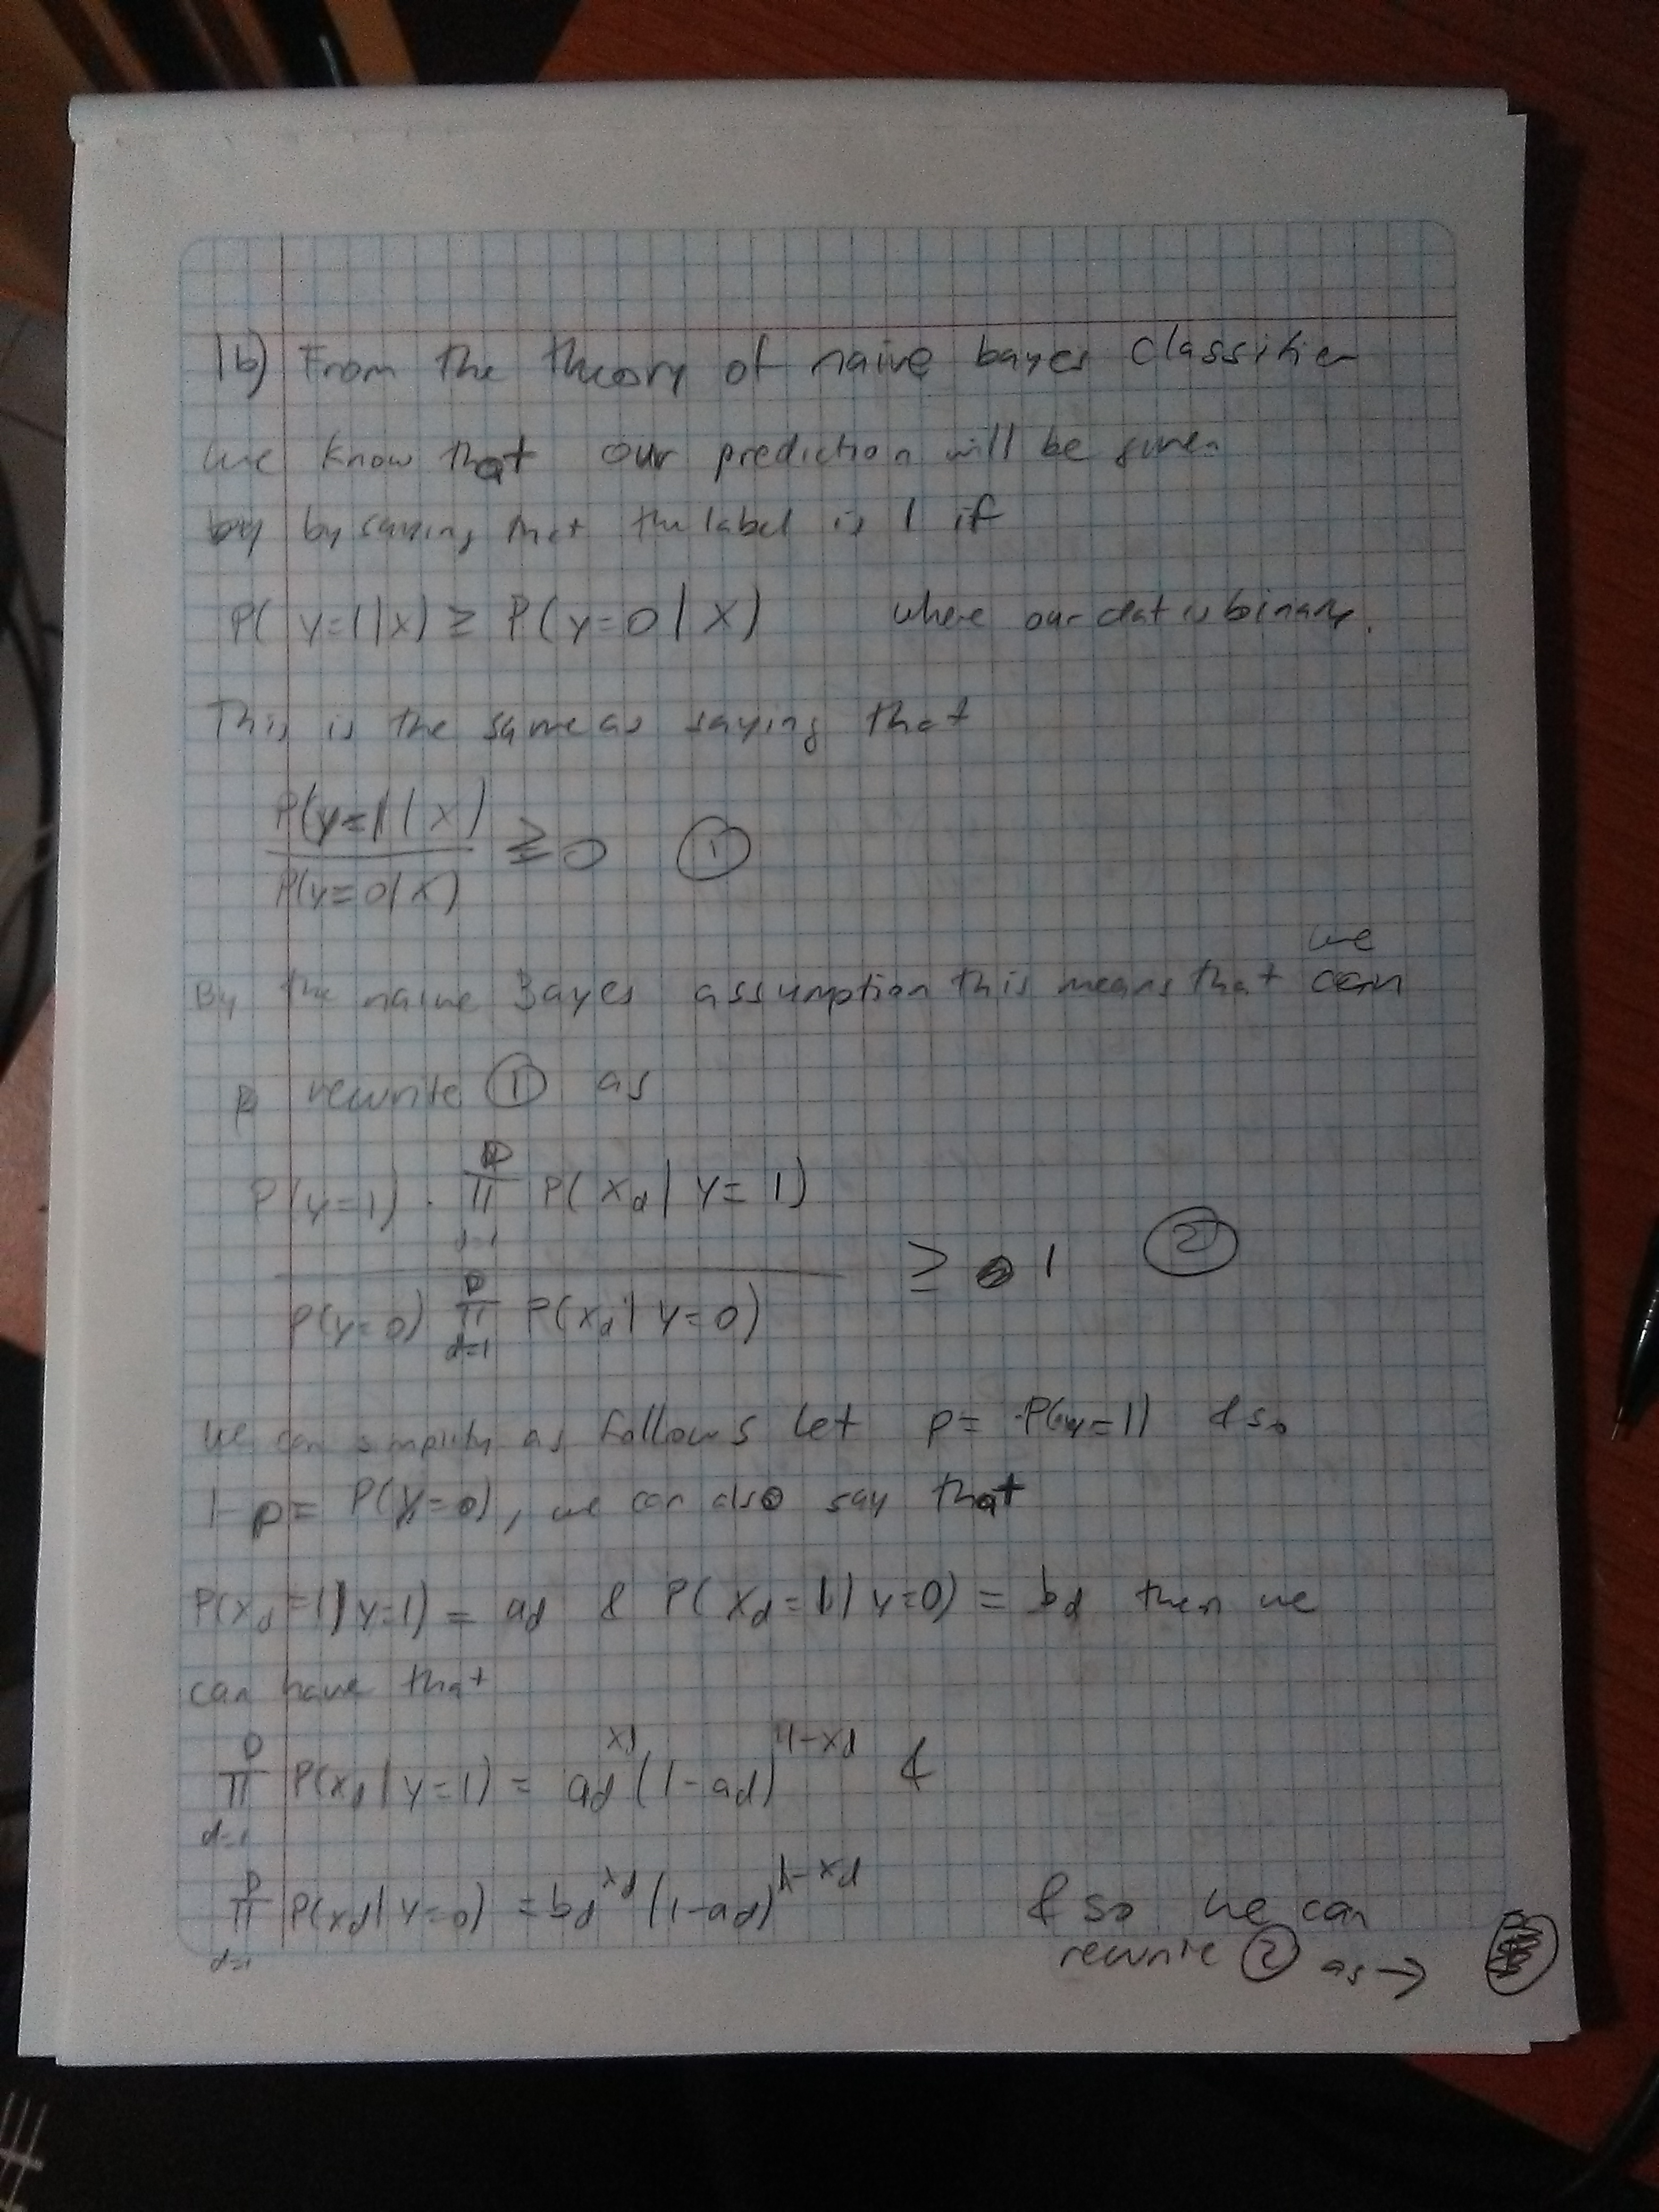
\includegraphics[width=10cm]{hw3_prob1b_1.jpg}
\caption{\textbf{Problem 1 part b:} Image showing the work done to show that the binary naive bayes classifier is a linear classifier}
\end{figure} 
\begin{figure}[!htbp]
\centering
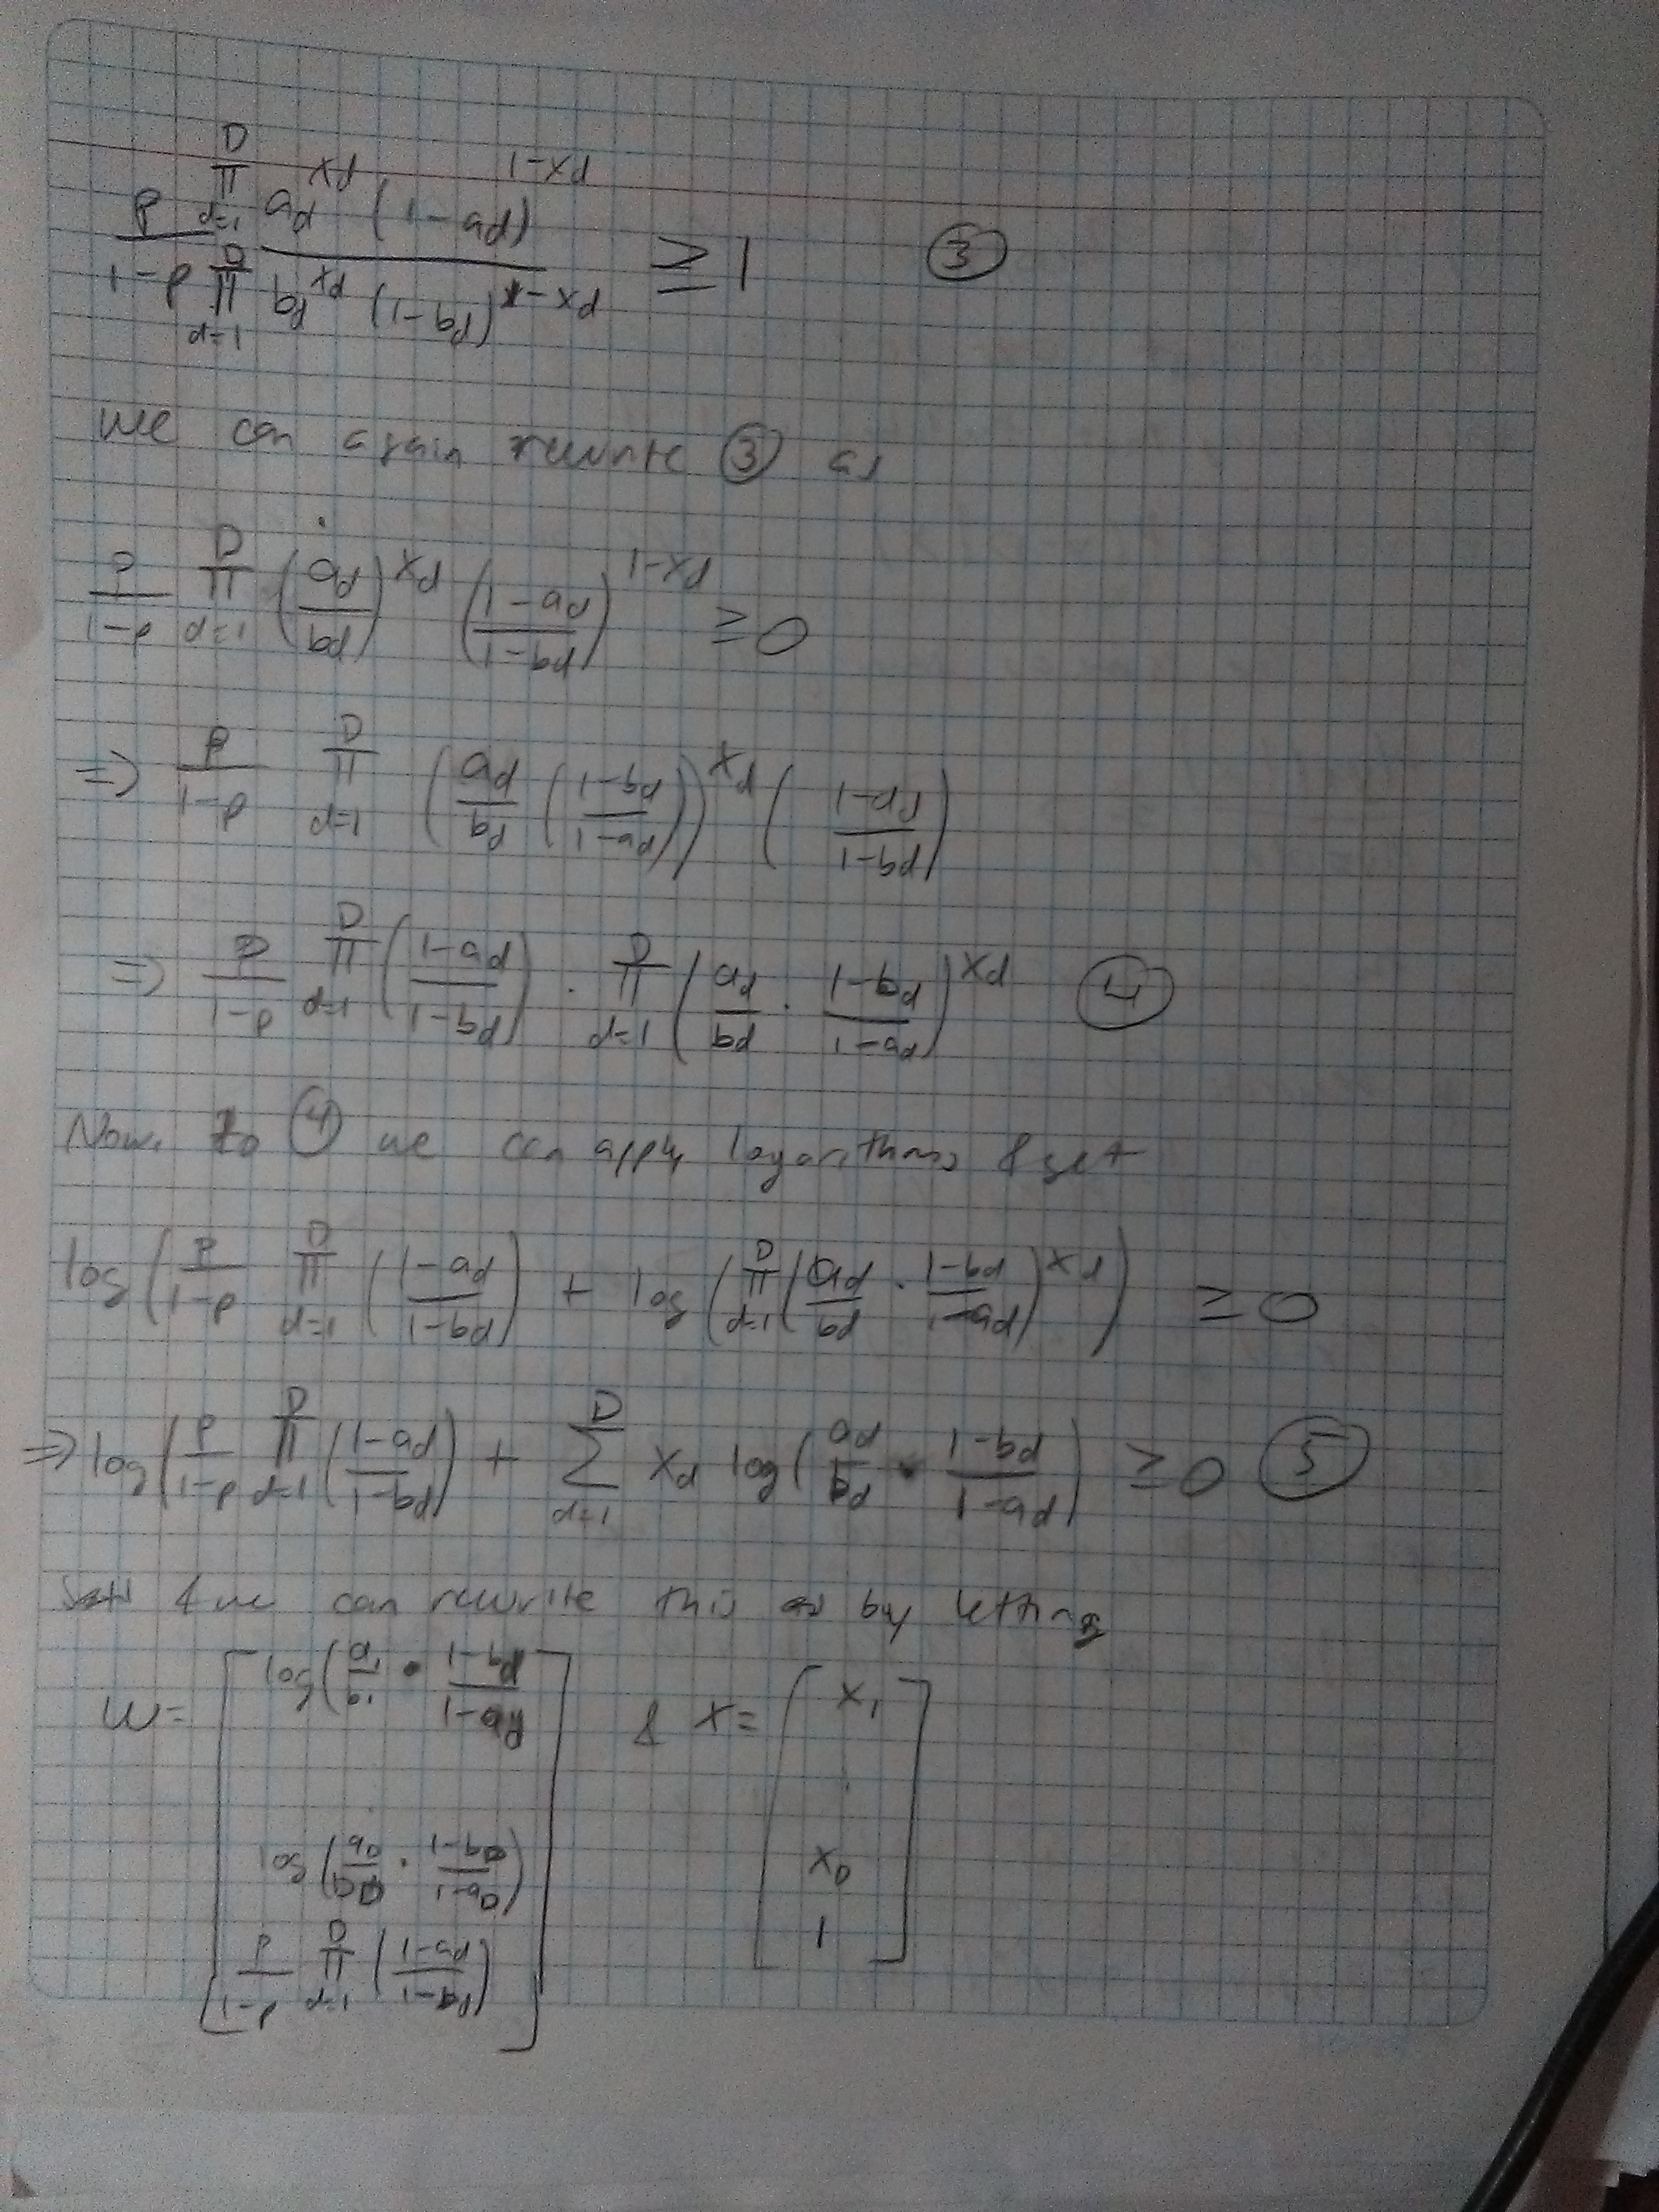
\includegraphics[width=10cm]{hw3_prob1b_2.jpg}
\caption{\textbf{Problem 1 part b:} Image showing the work done to show that the binary naive bayes classifier is a linear classifier}
\end{figure} 
\begin{figure}[!htbp]
\centering
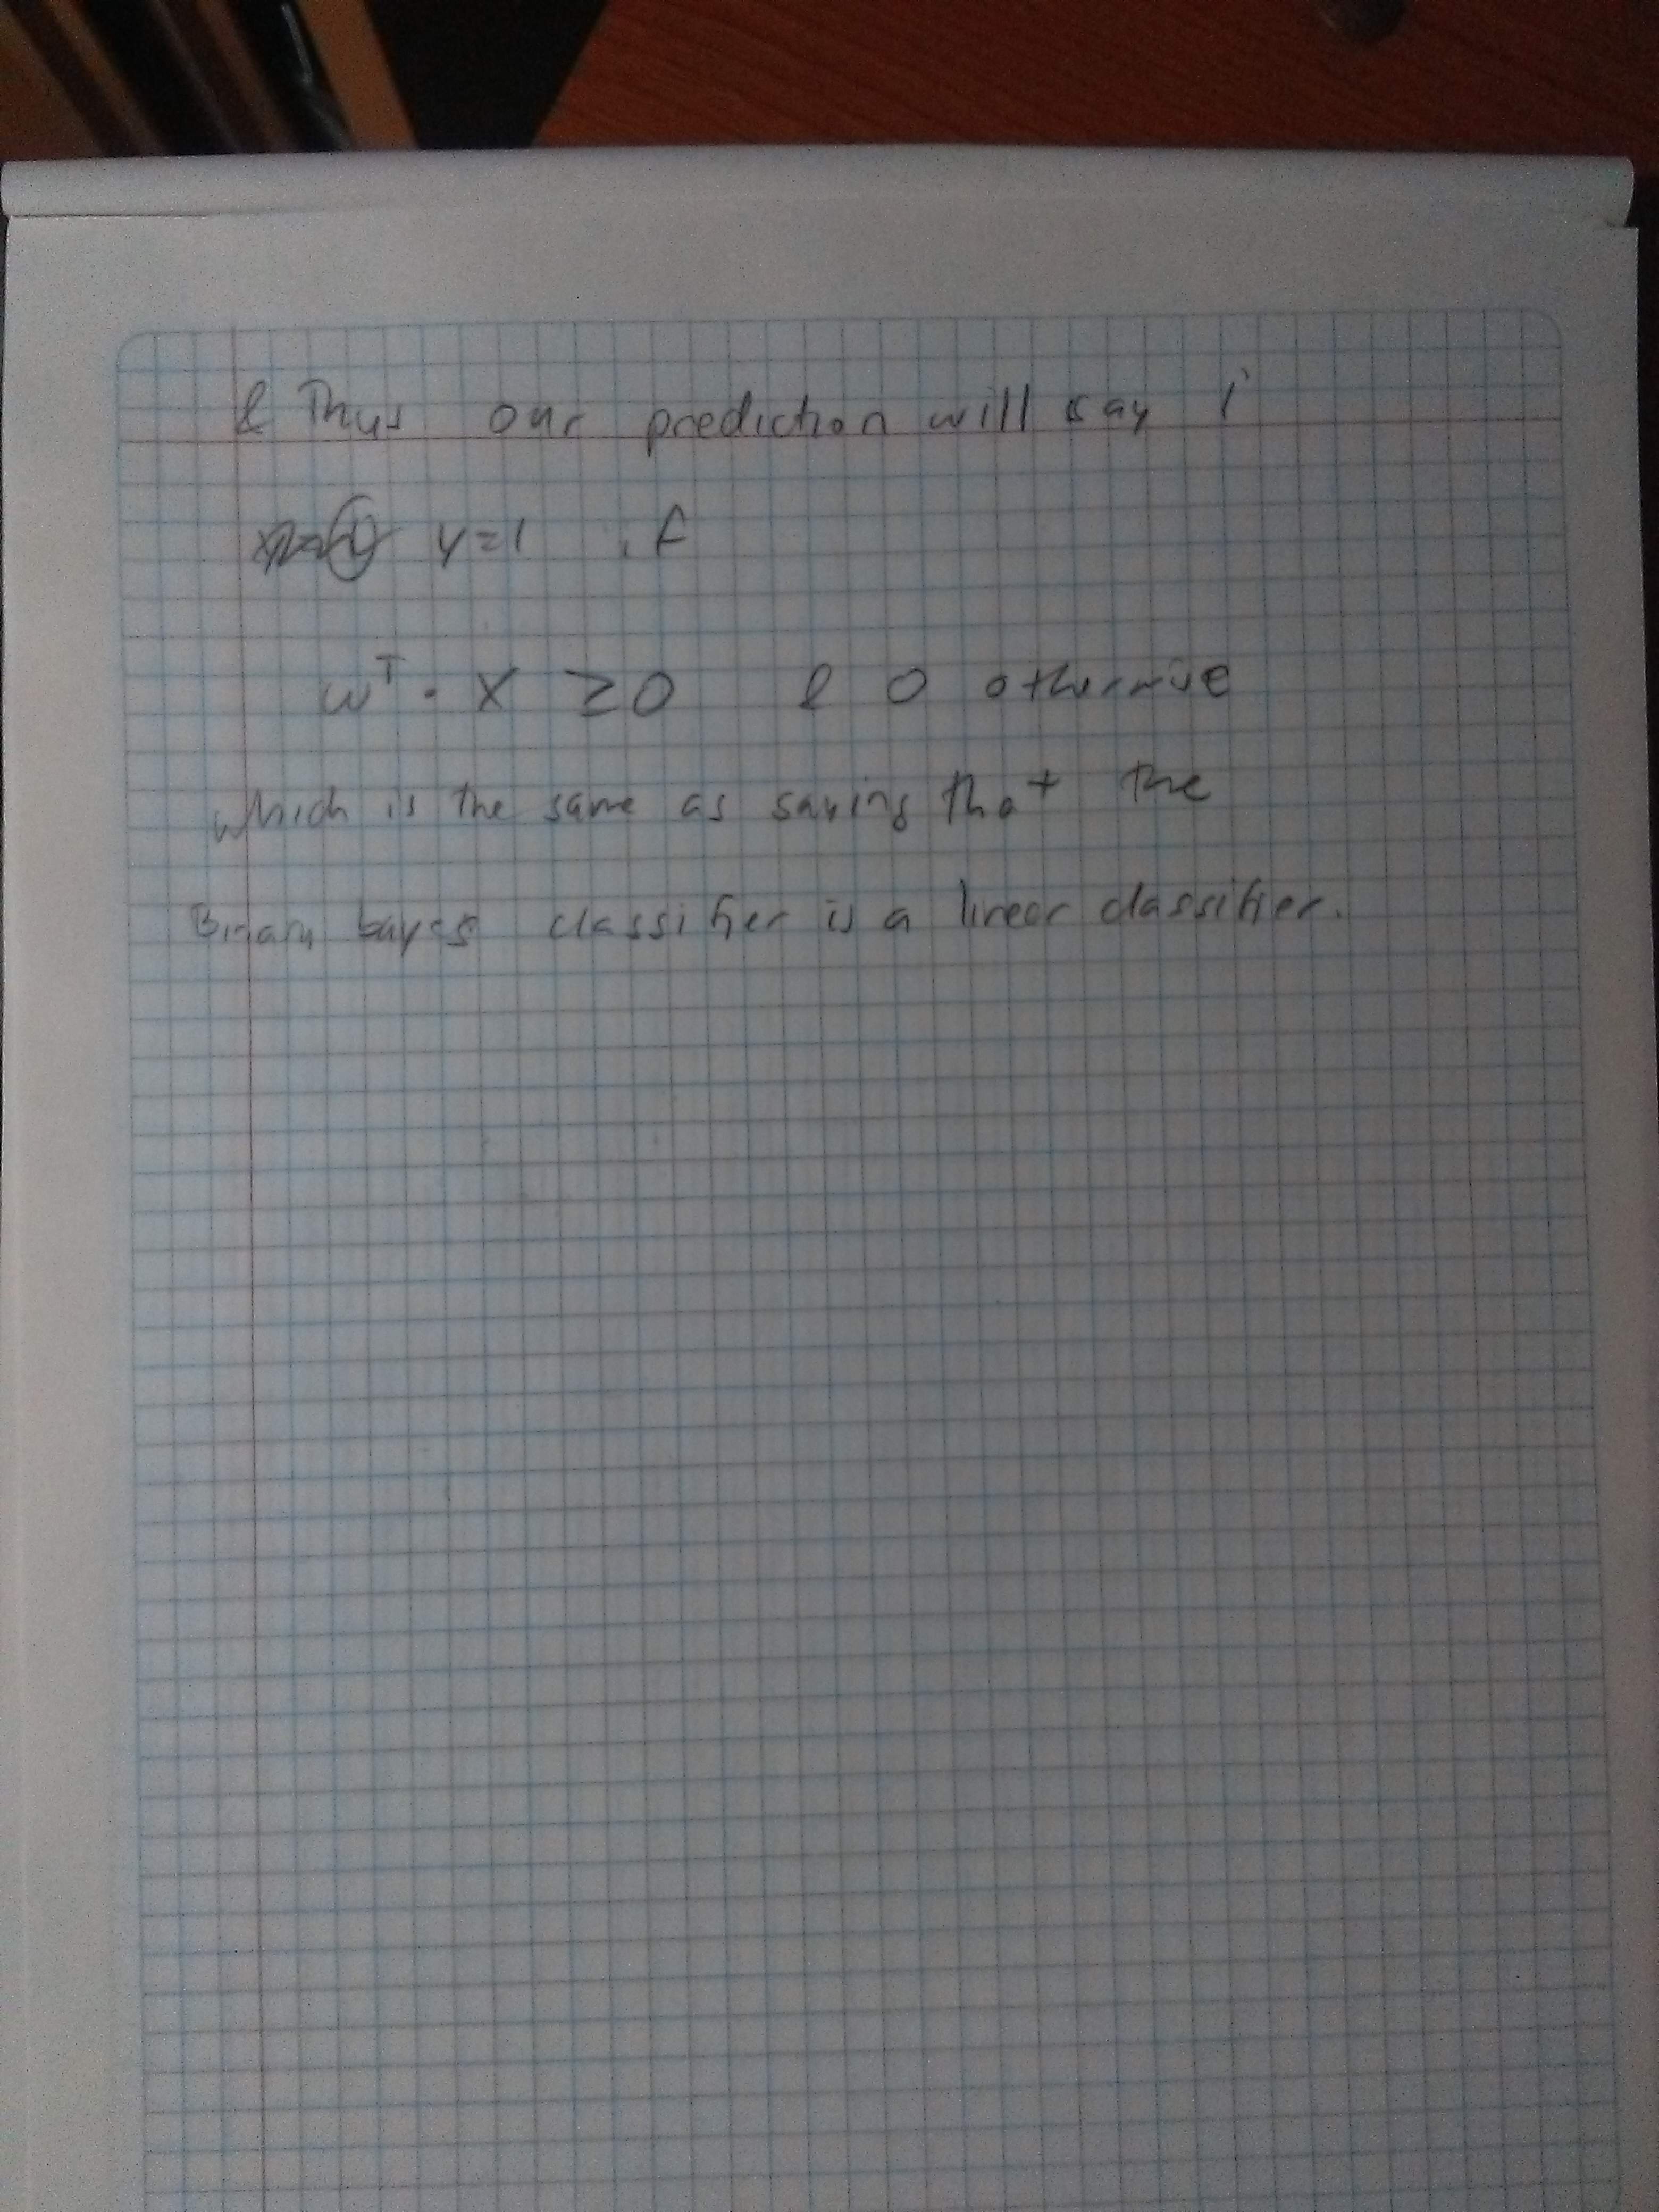
\includegraphics[width=10cm]{hw3_prob1b_3.jpg}
\caption{\textbf{Problem 1 part b:} Image showing the work done to show that the binary naive bayes classifier is a linear classifier}
\end{figure} 

\end{enumerate}

\end{proof}

\begin{problem}
\normalfont
Problem 2
\end{problem}

\begin{proof}
The solution to this problem is presented in the following pictures.


\begin{figure}[!htbp]
\centering
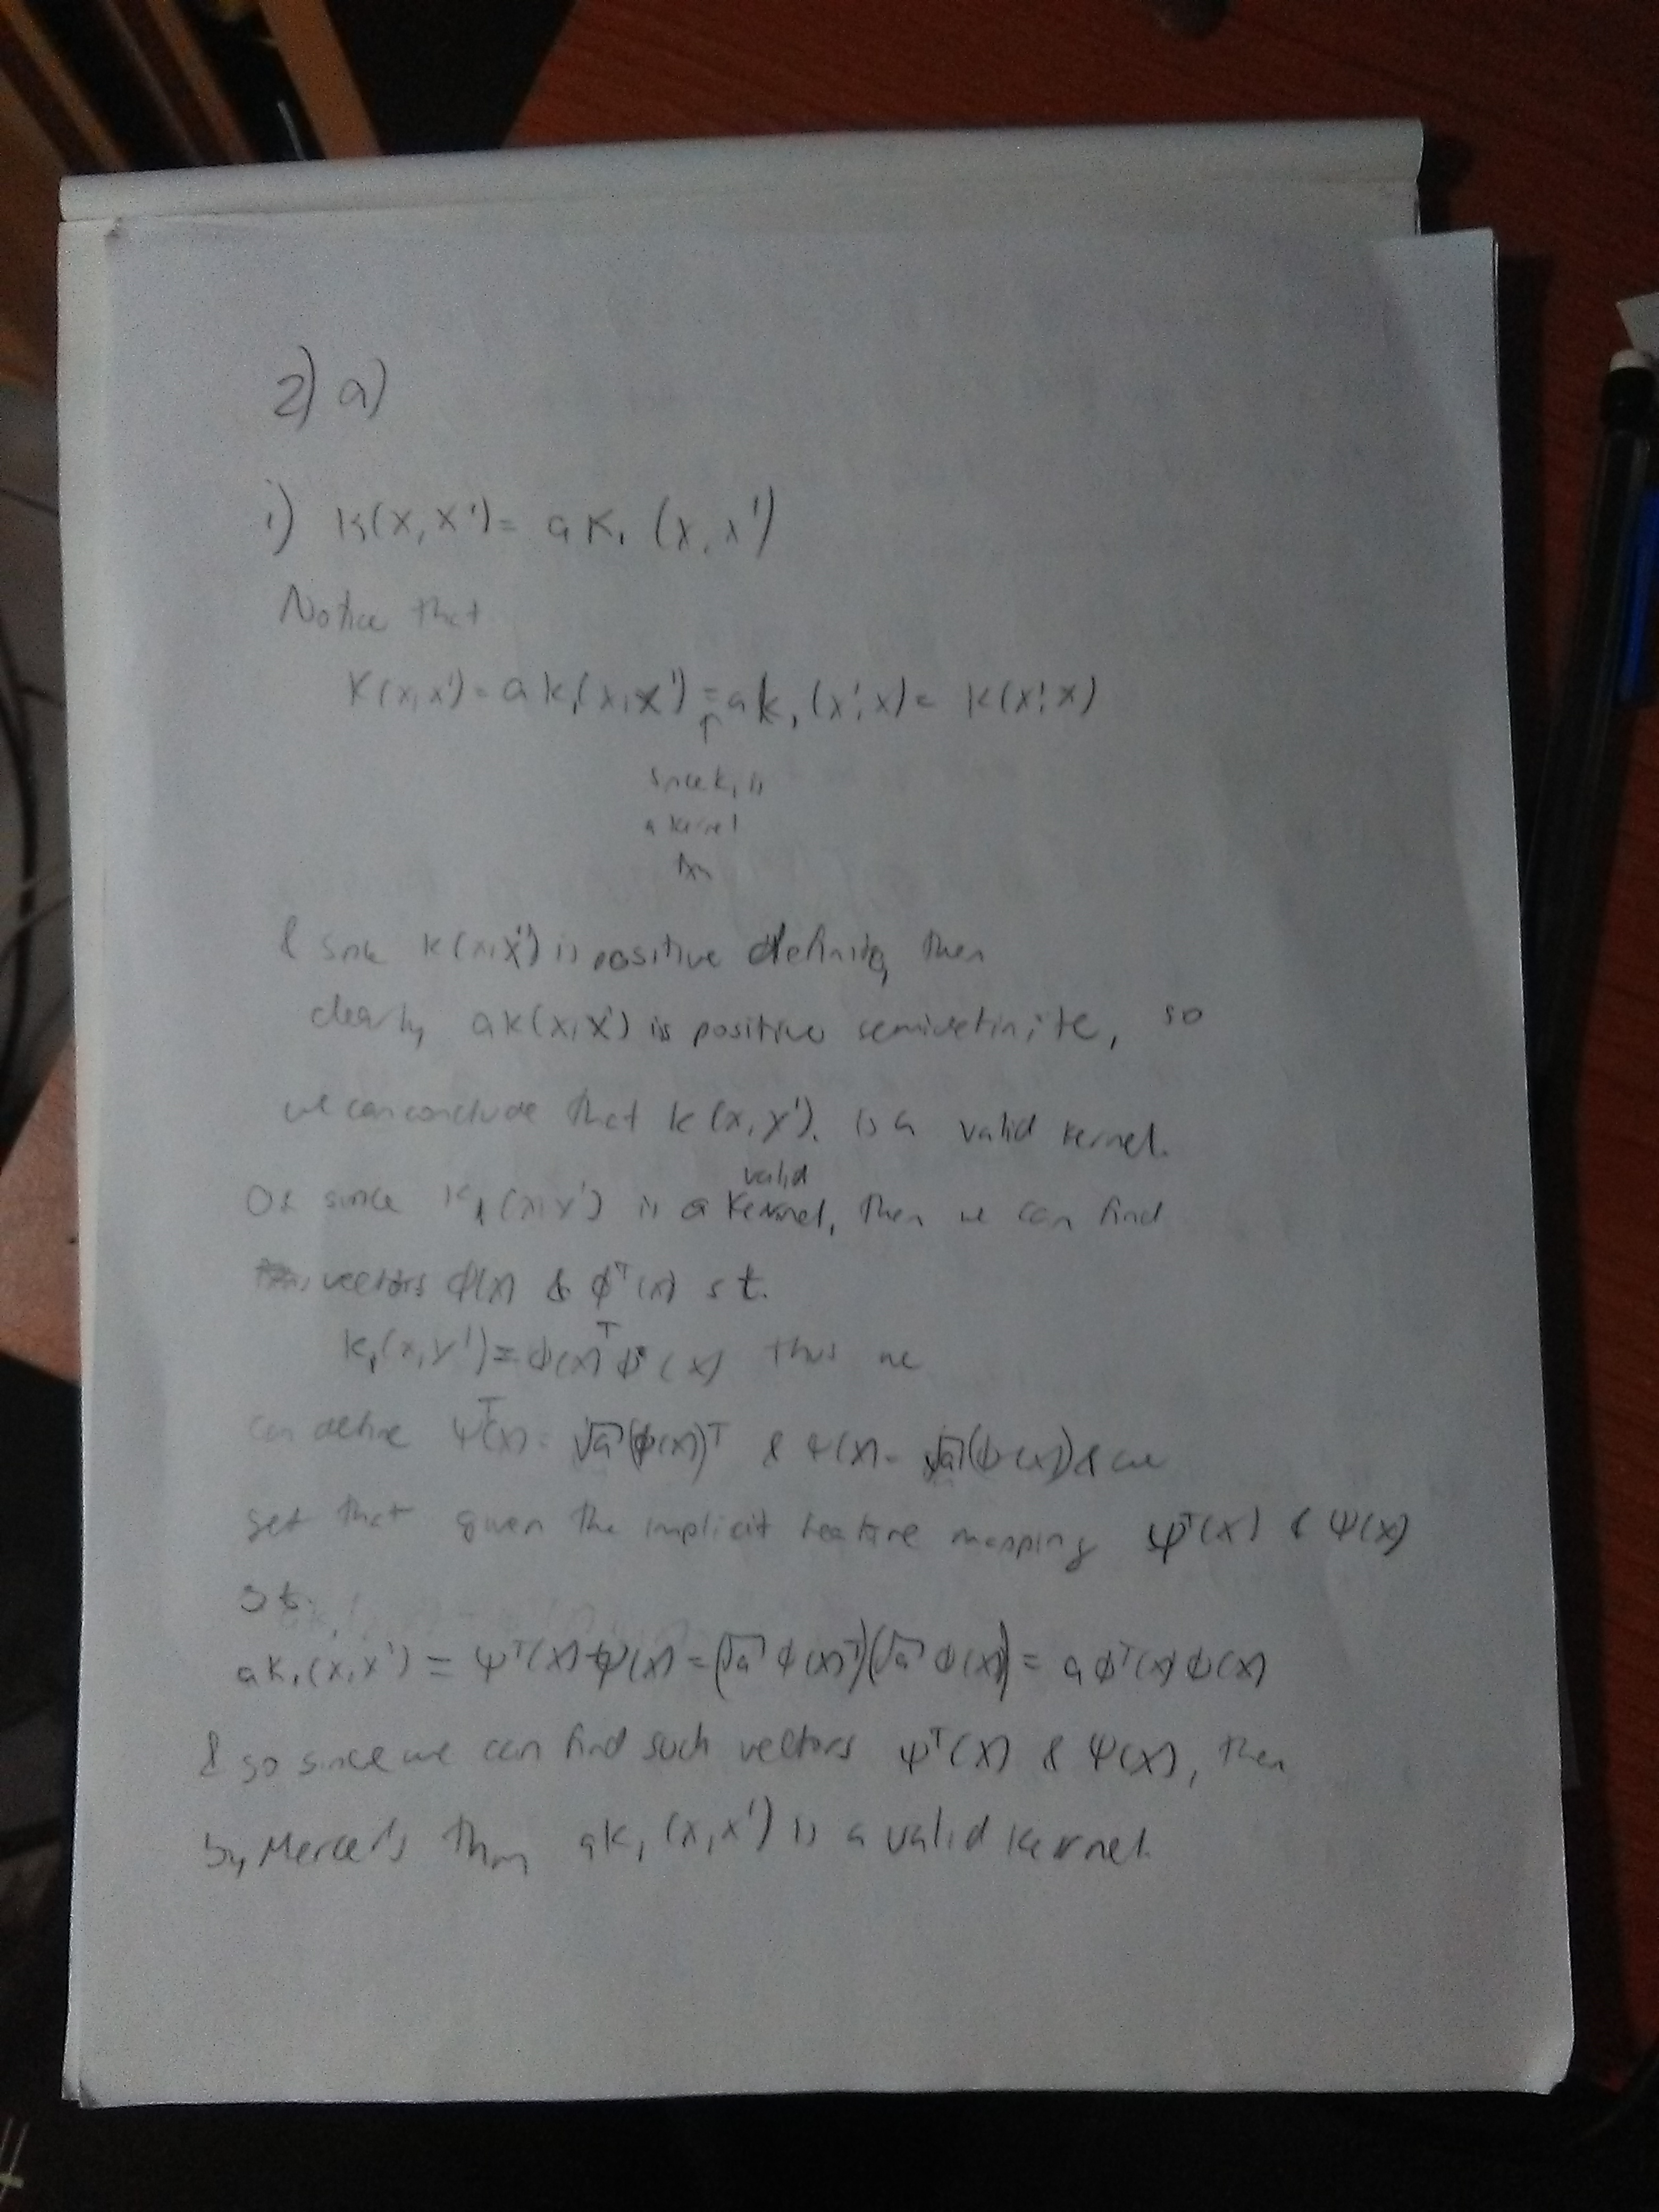
\includegraphics[width=10cm]{hw3_prob2a_1.jpg}
\caption{\textbf{Problem 2a part 1:} Image showing the work for part 1 of problem 2a}
\end{figure}

\begin{figure}[!htbp]
\centering
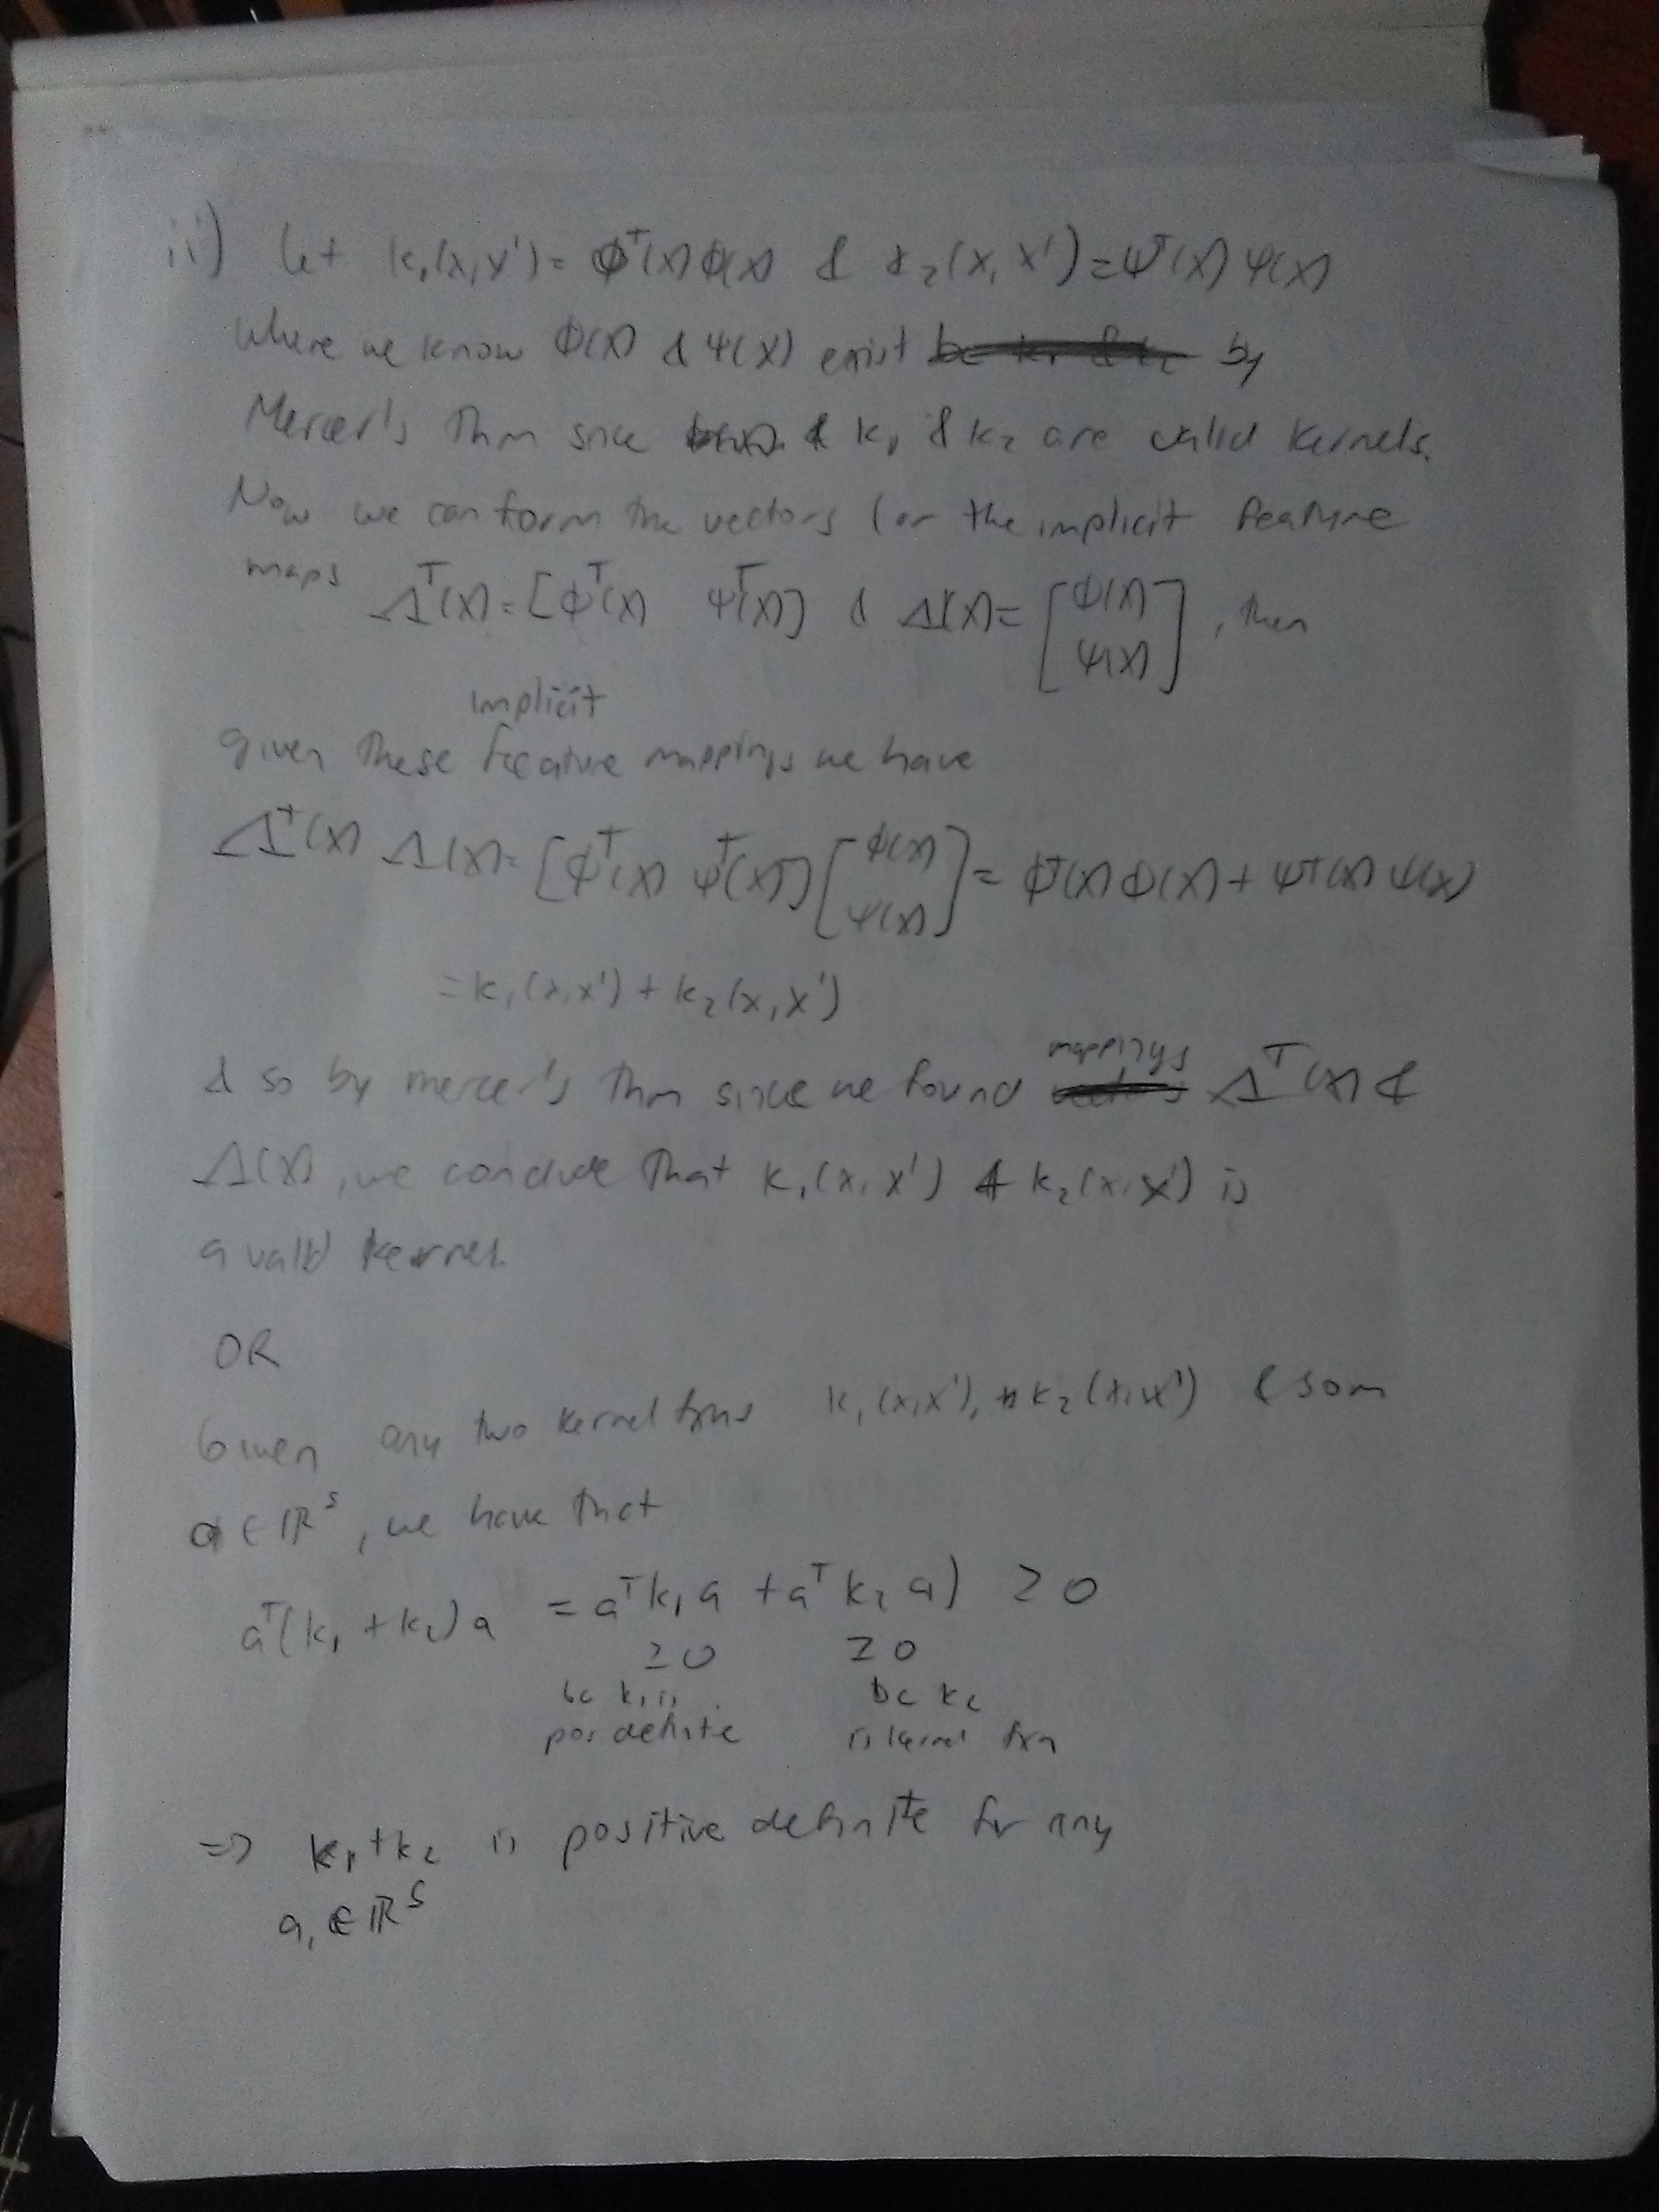
\includegraphics[width=10cm]{hw3_prob2a_2.jpg}
\caption{\textbf{Problem 2a part 2:} Image showing the work for part 2 of problem 2a}
\end{figure}

\begin{figure}[!htbp]
\centering
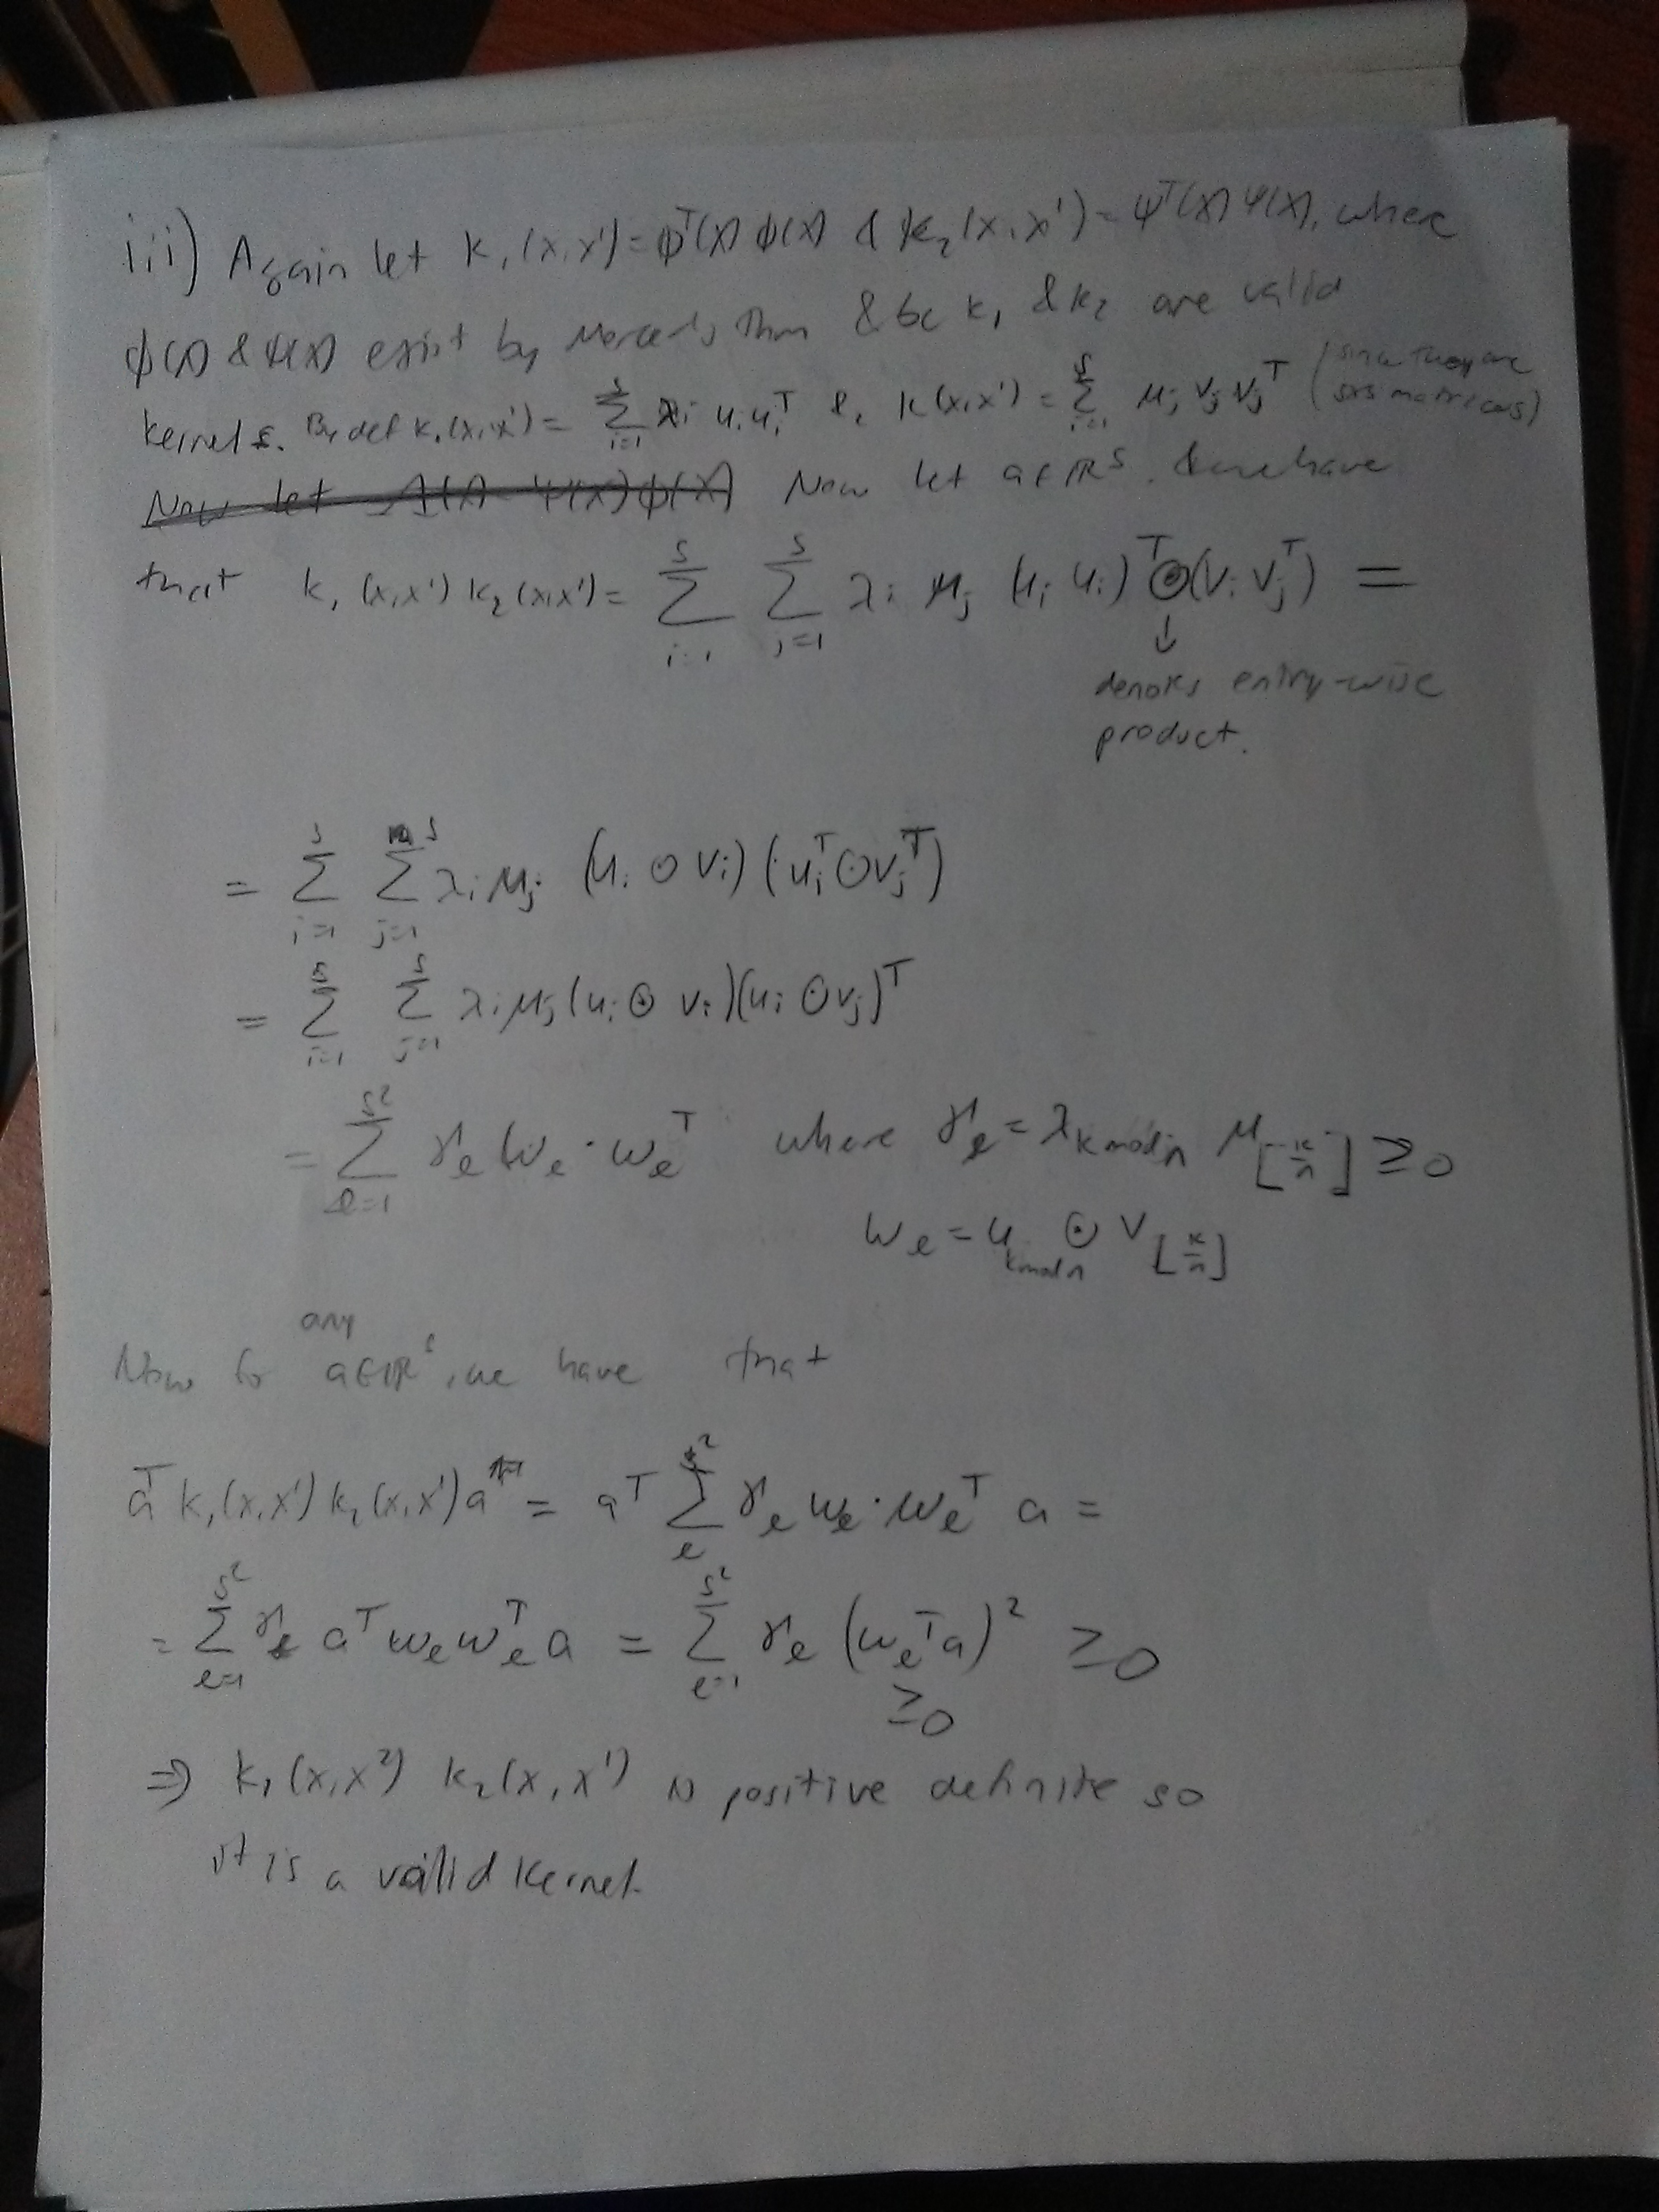
\includegraphics[width=10cm]{hw3_prob2a_3.jpg}
\caption{\textbf{Problem 2a part 3:} Image showing the work for part 3 of problem 2a}
\end{figure}

\begin{figure}[!htbp]
\centering
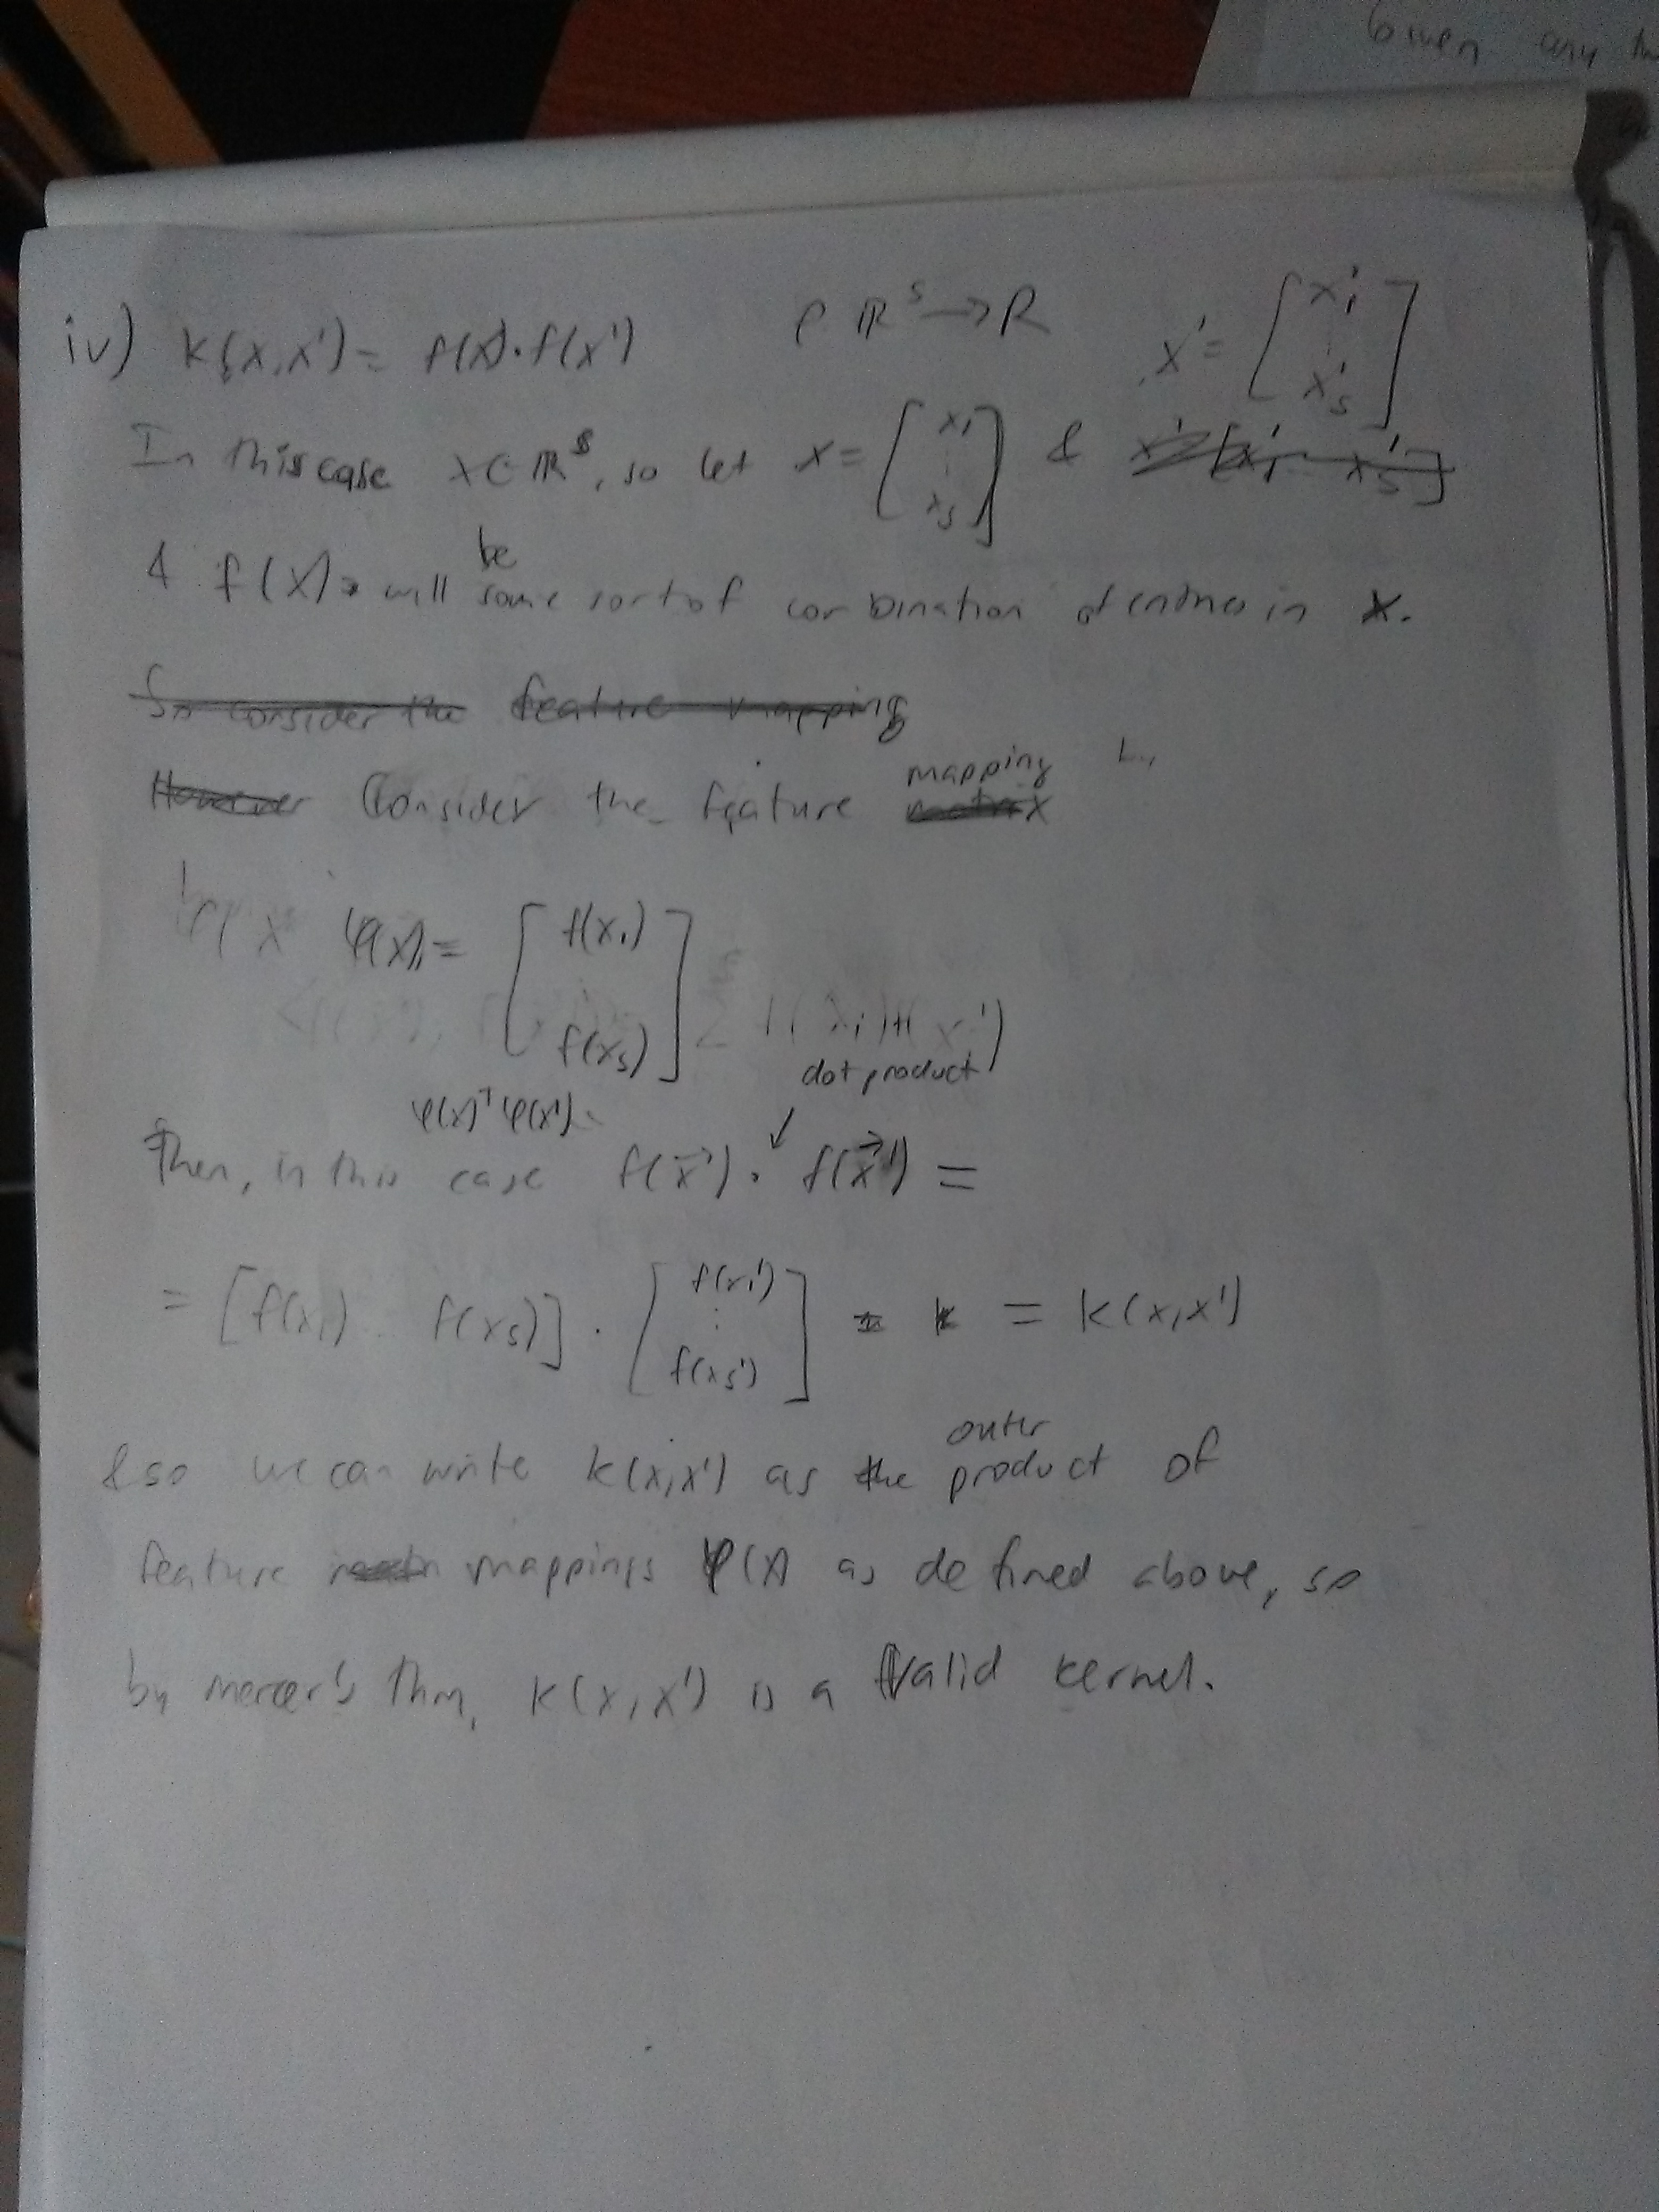
\includegraphics[width=10cm]{hw3_prob2a_4.jpg}
\caption{\textbf{Problem 2a part 4:} Image showing the work for part 4 of problem 2a}
\end{figure}

\begin{figure}[!htbp]
\centering
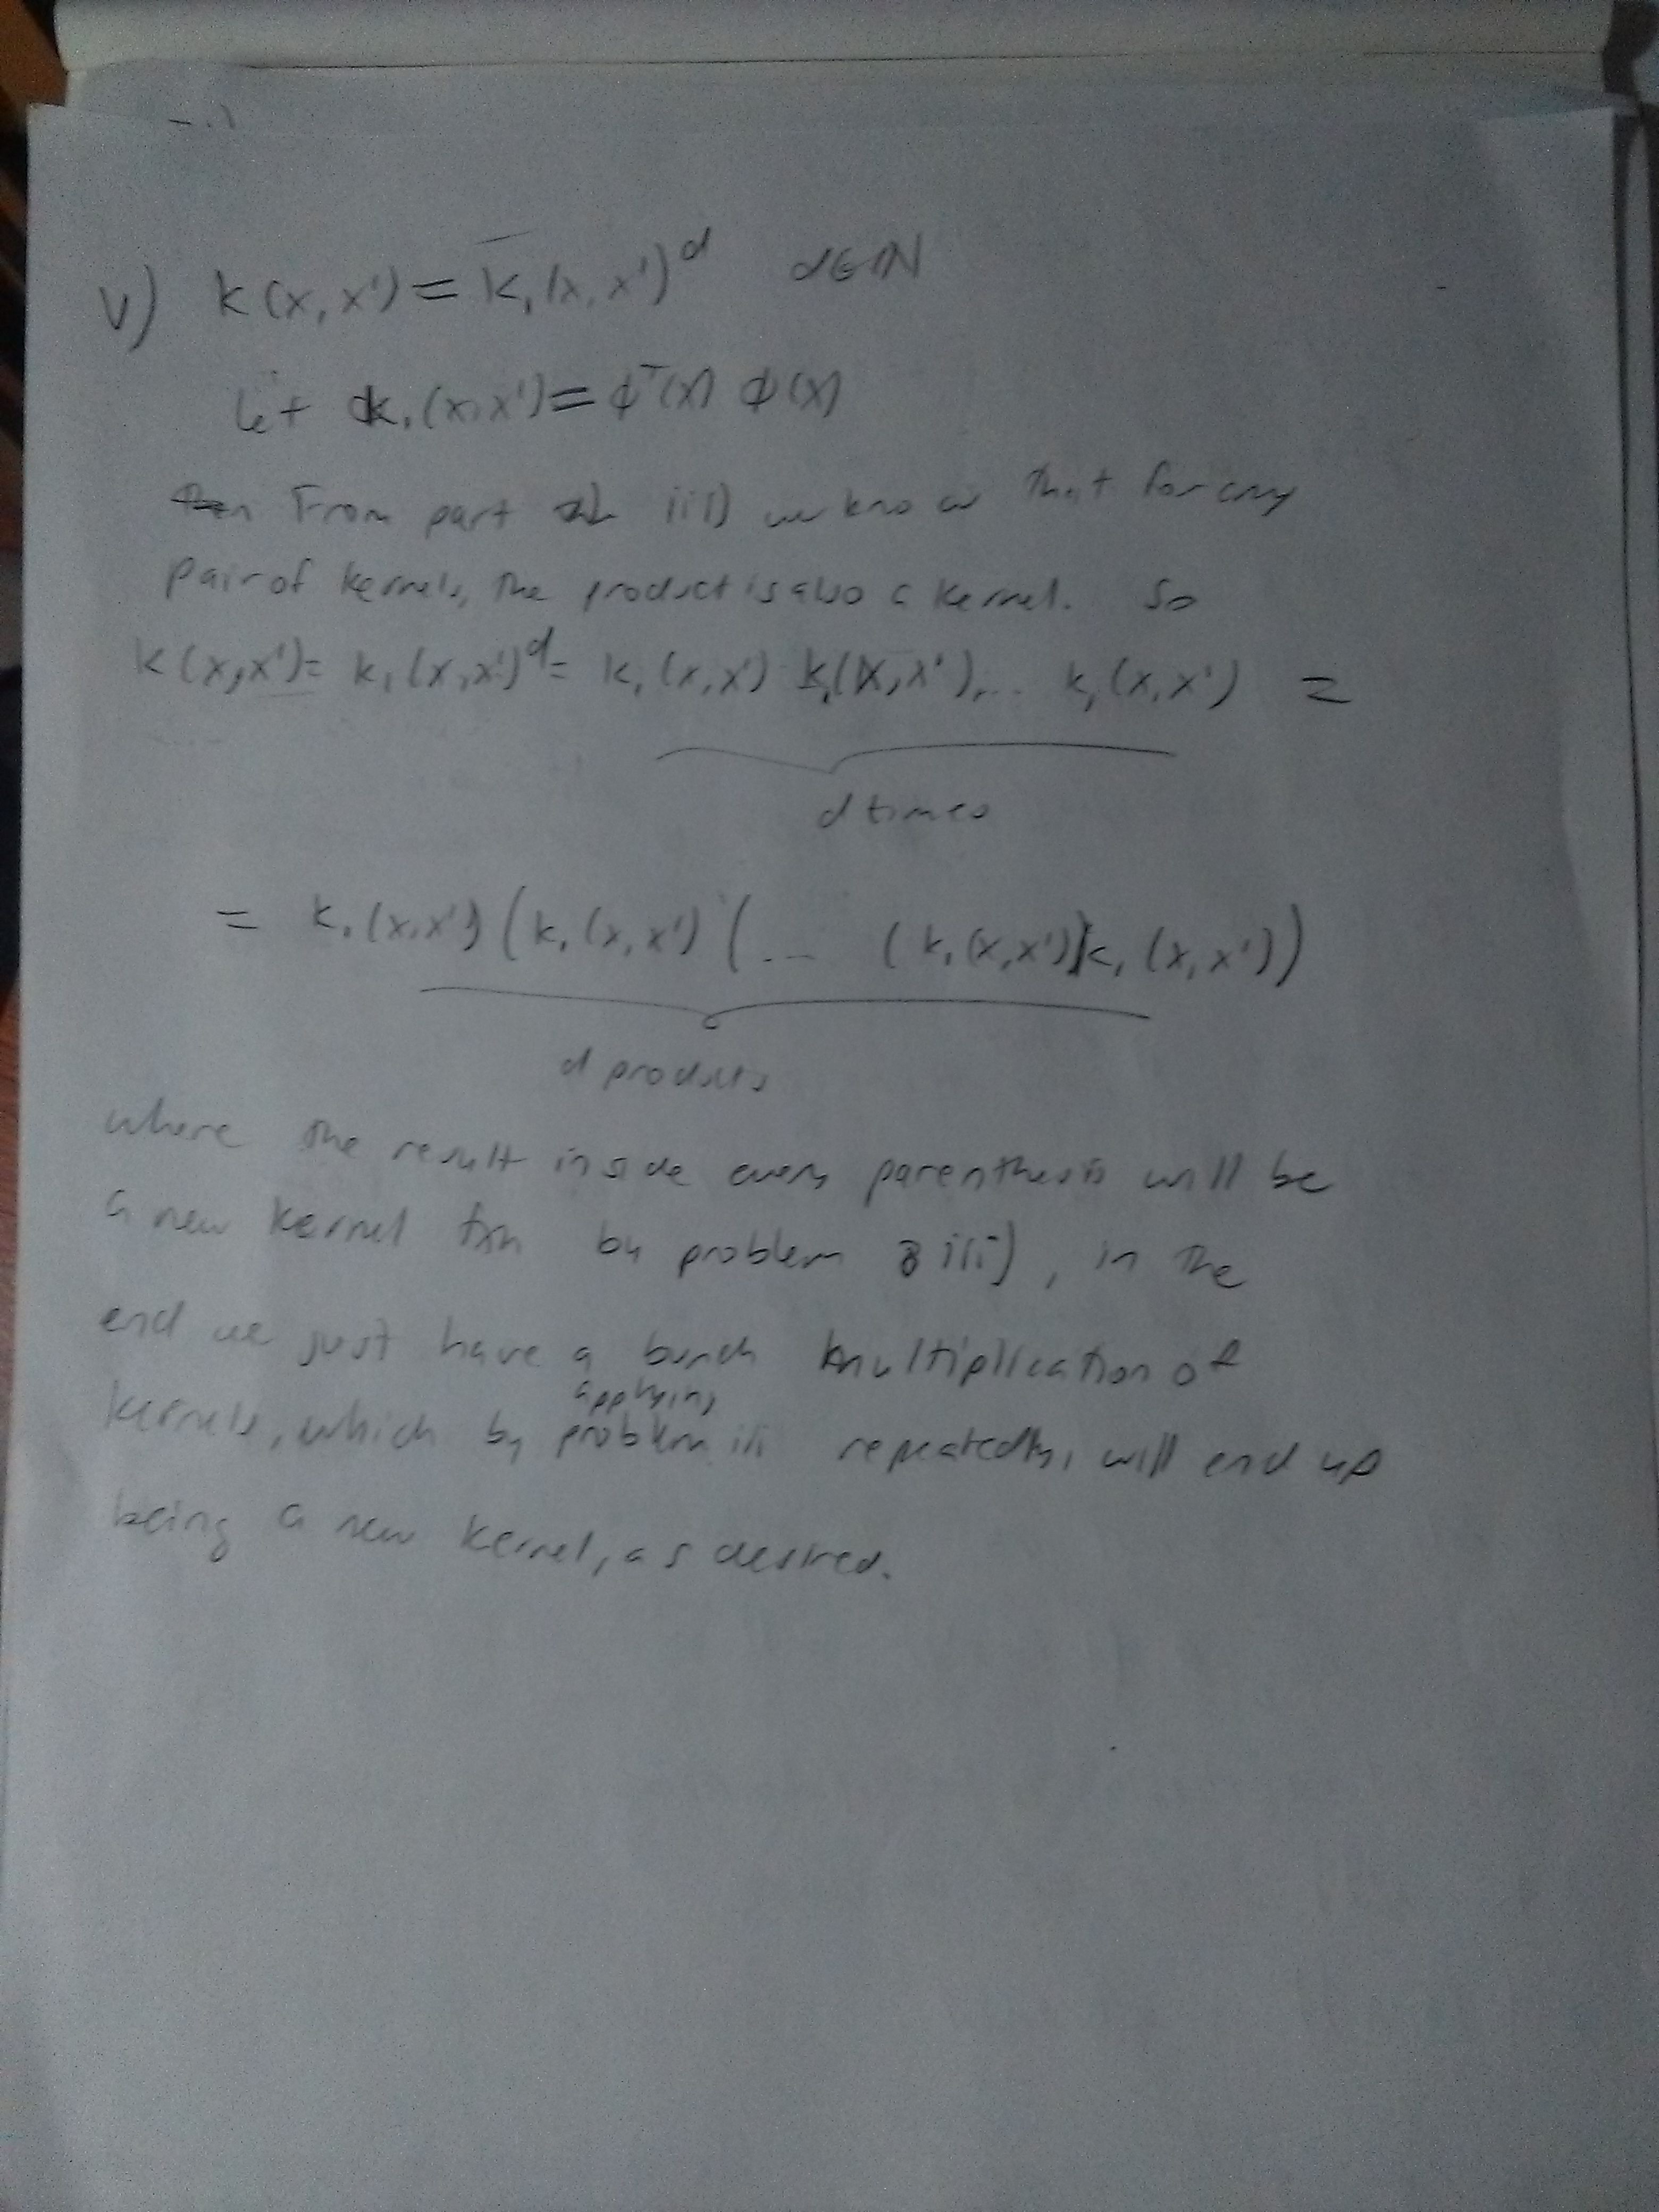
\includegraphics[width=10cm]{hw3_prob2a_5.jpg}
\caption{\textbf{Problem 2a part 5:} Image showing the work for part 5 of problem 2a}
\end{figure}

\begin{figure}[!htbp]
\centering
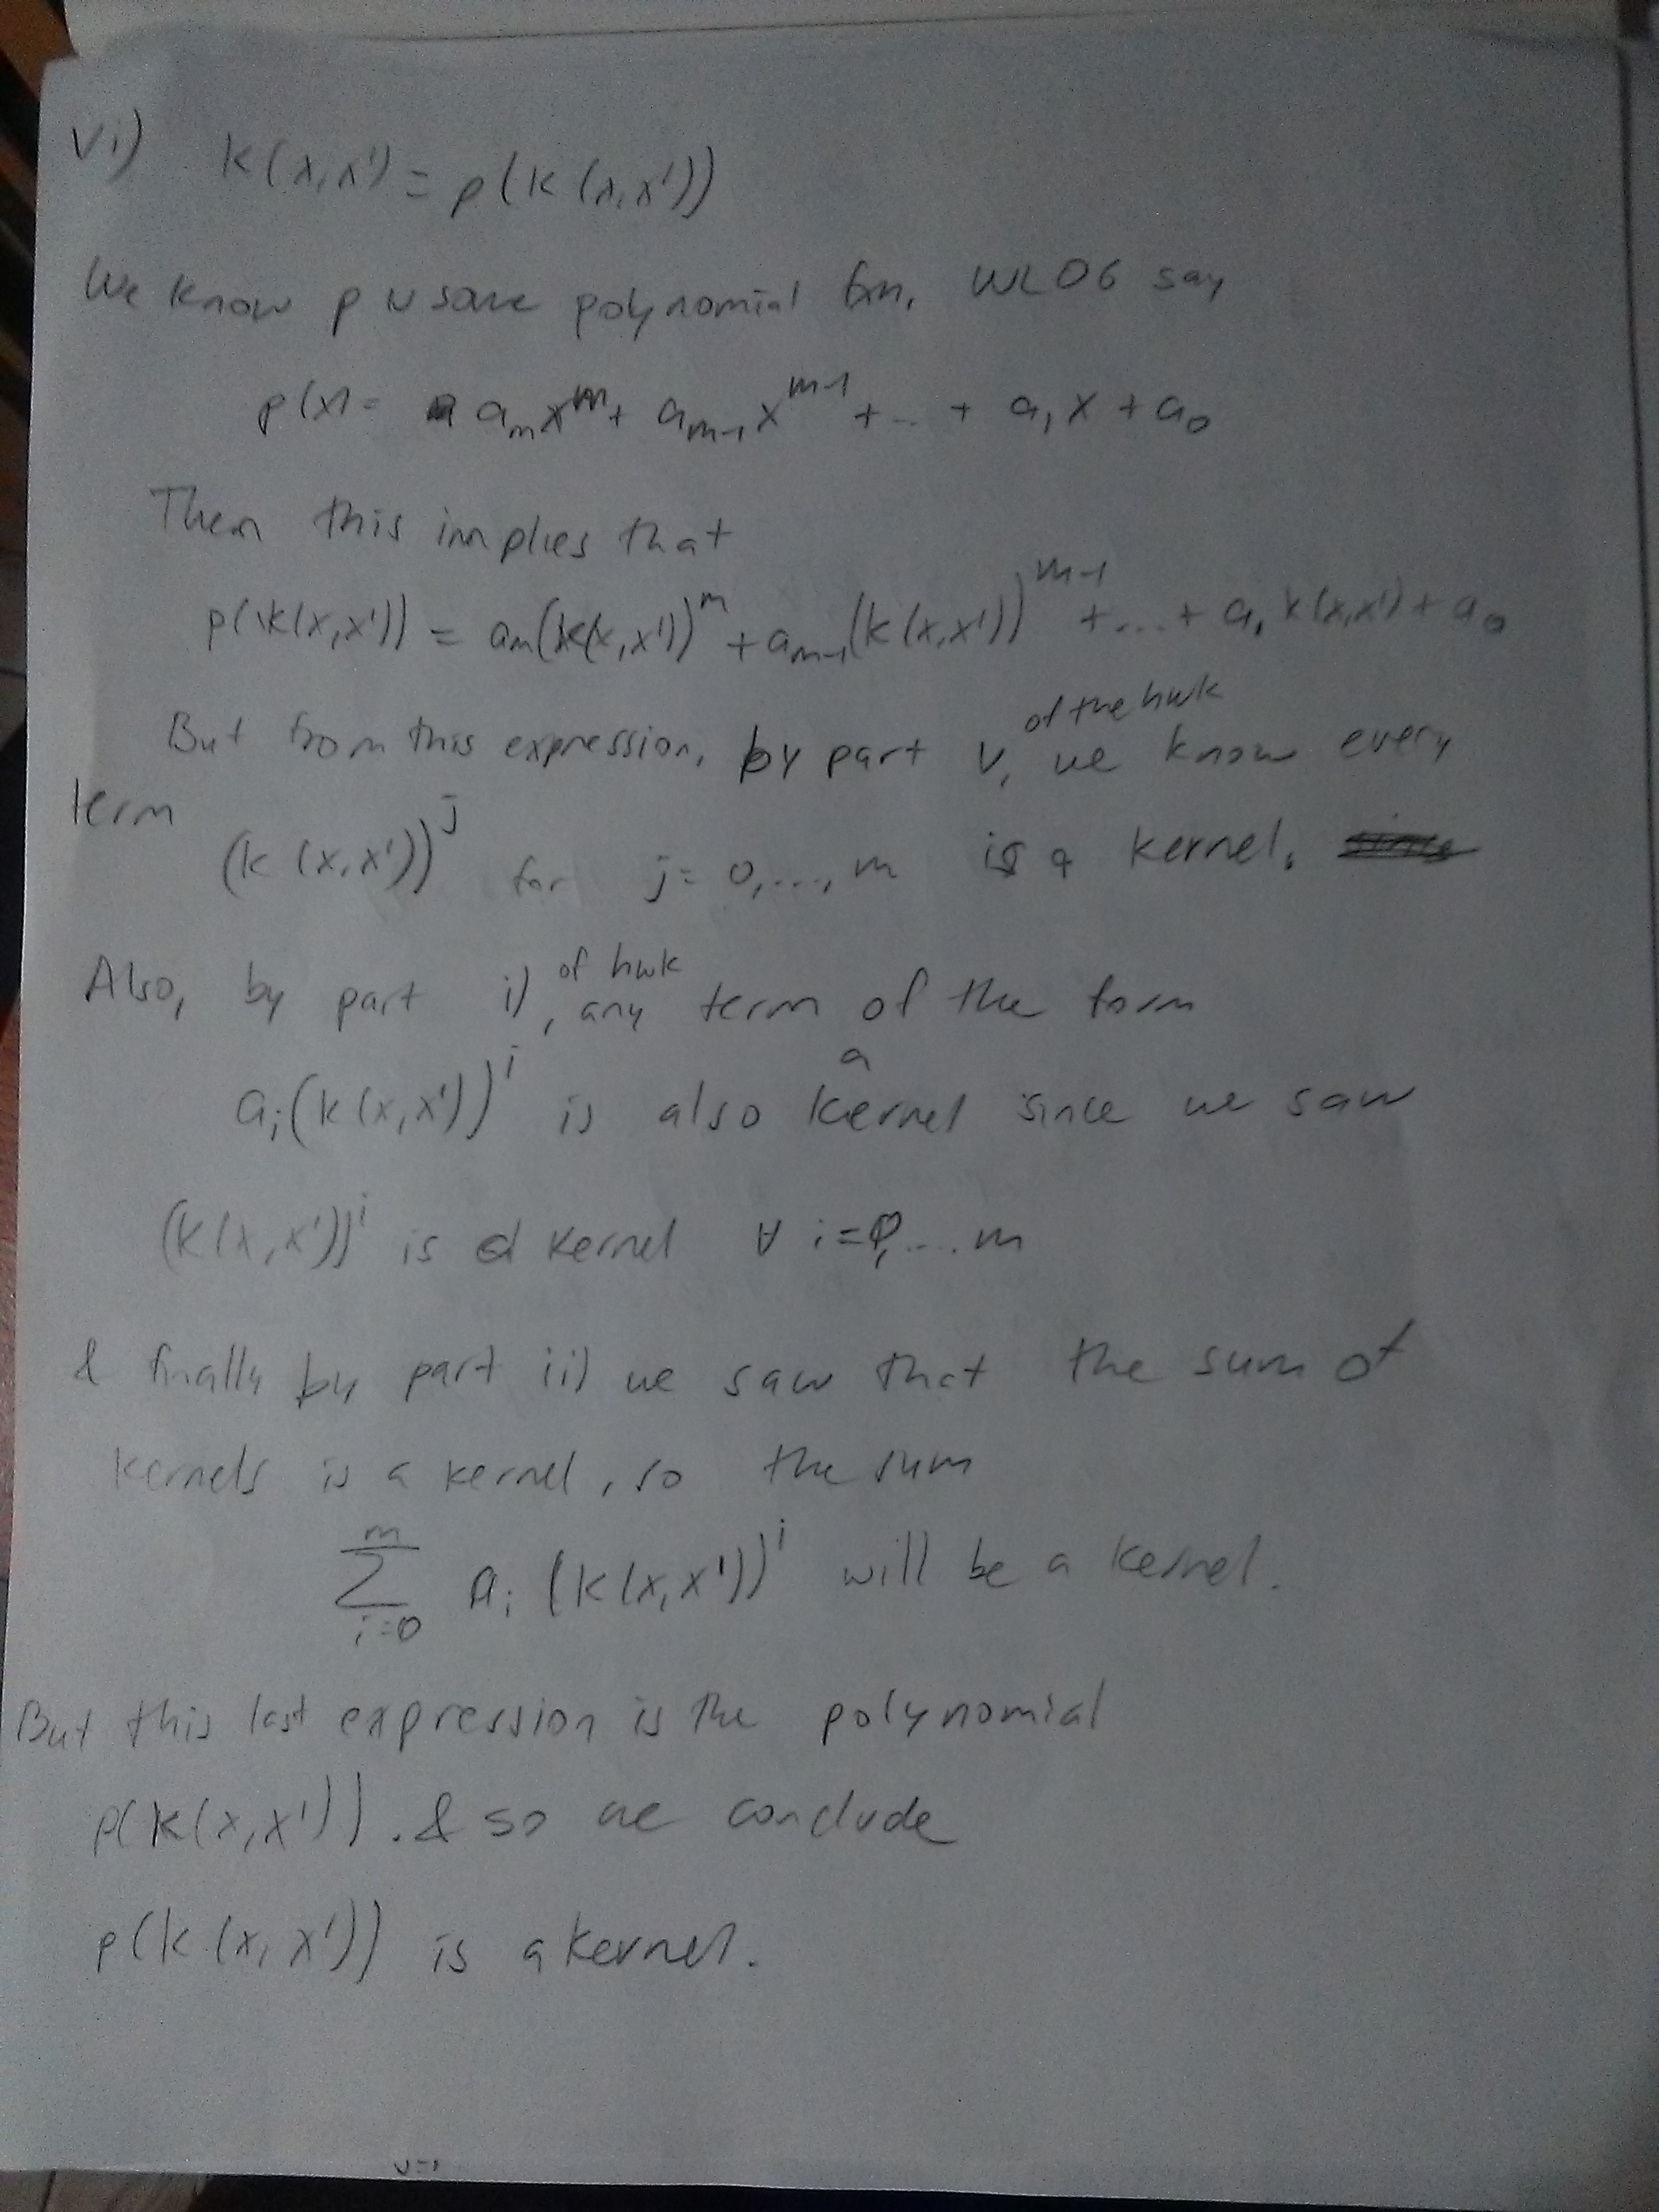
\includegraphics[width=10cm]{hw3_prob2a_6.jpg}
\caption{\textbf{Problem 2a part 6:} Image showing the work for part 6 of problem 2a}
\end{figure}

 Now, we show the solution for \textbf{problem 2 part b}
\begin{figure}[!htbp]
\centering
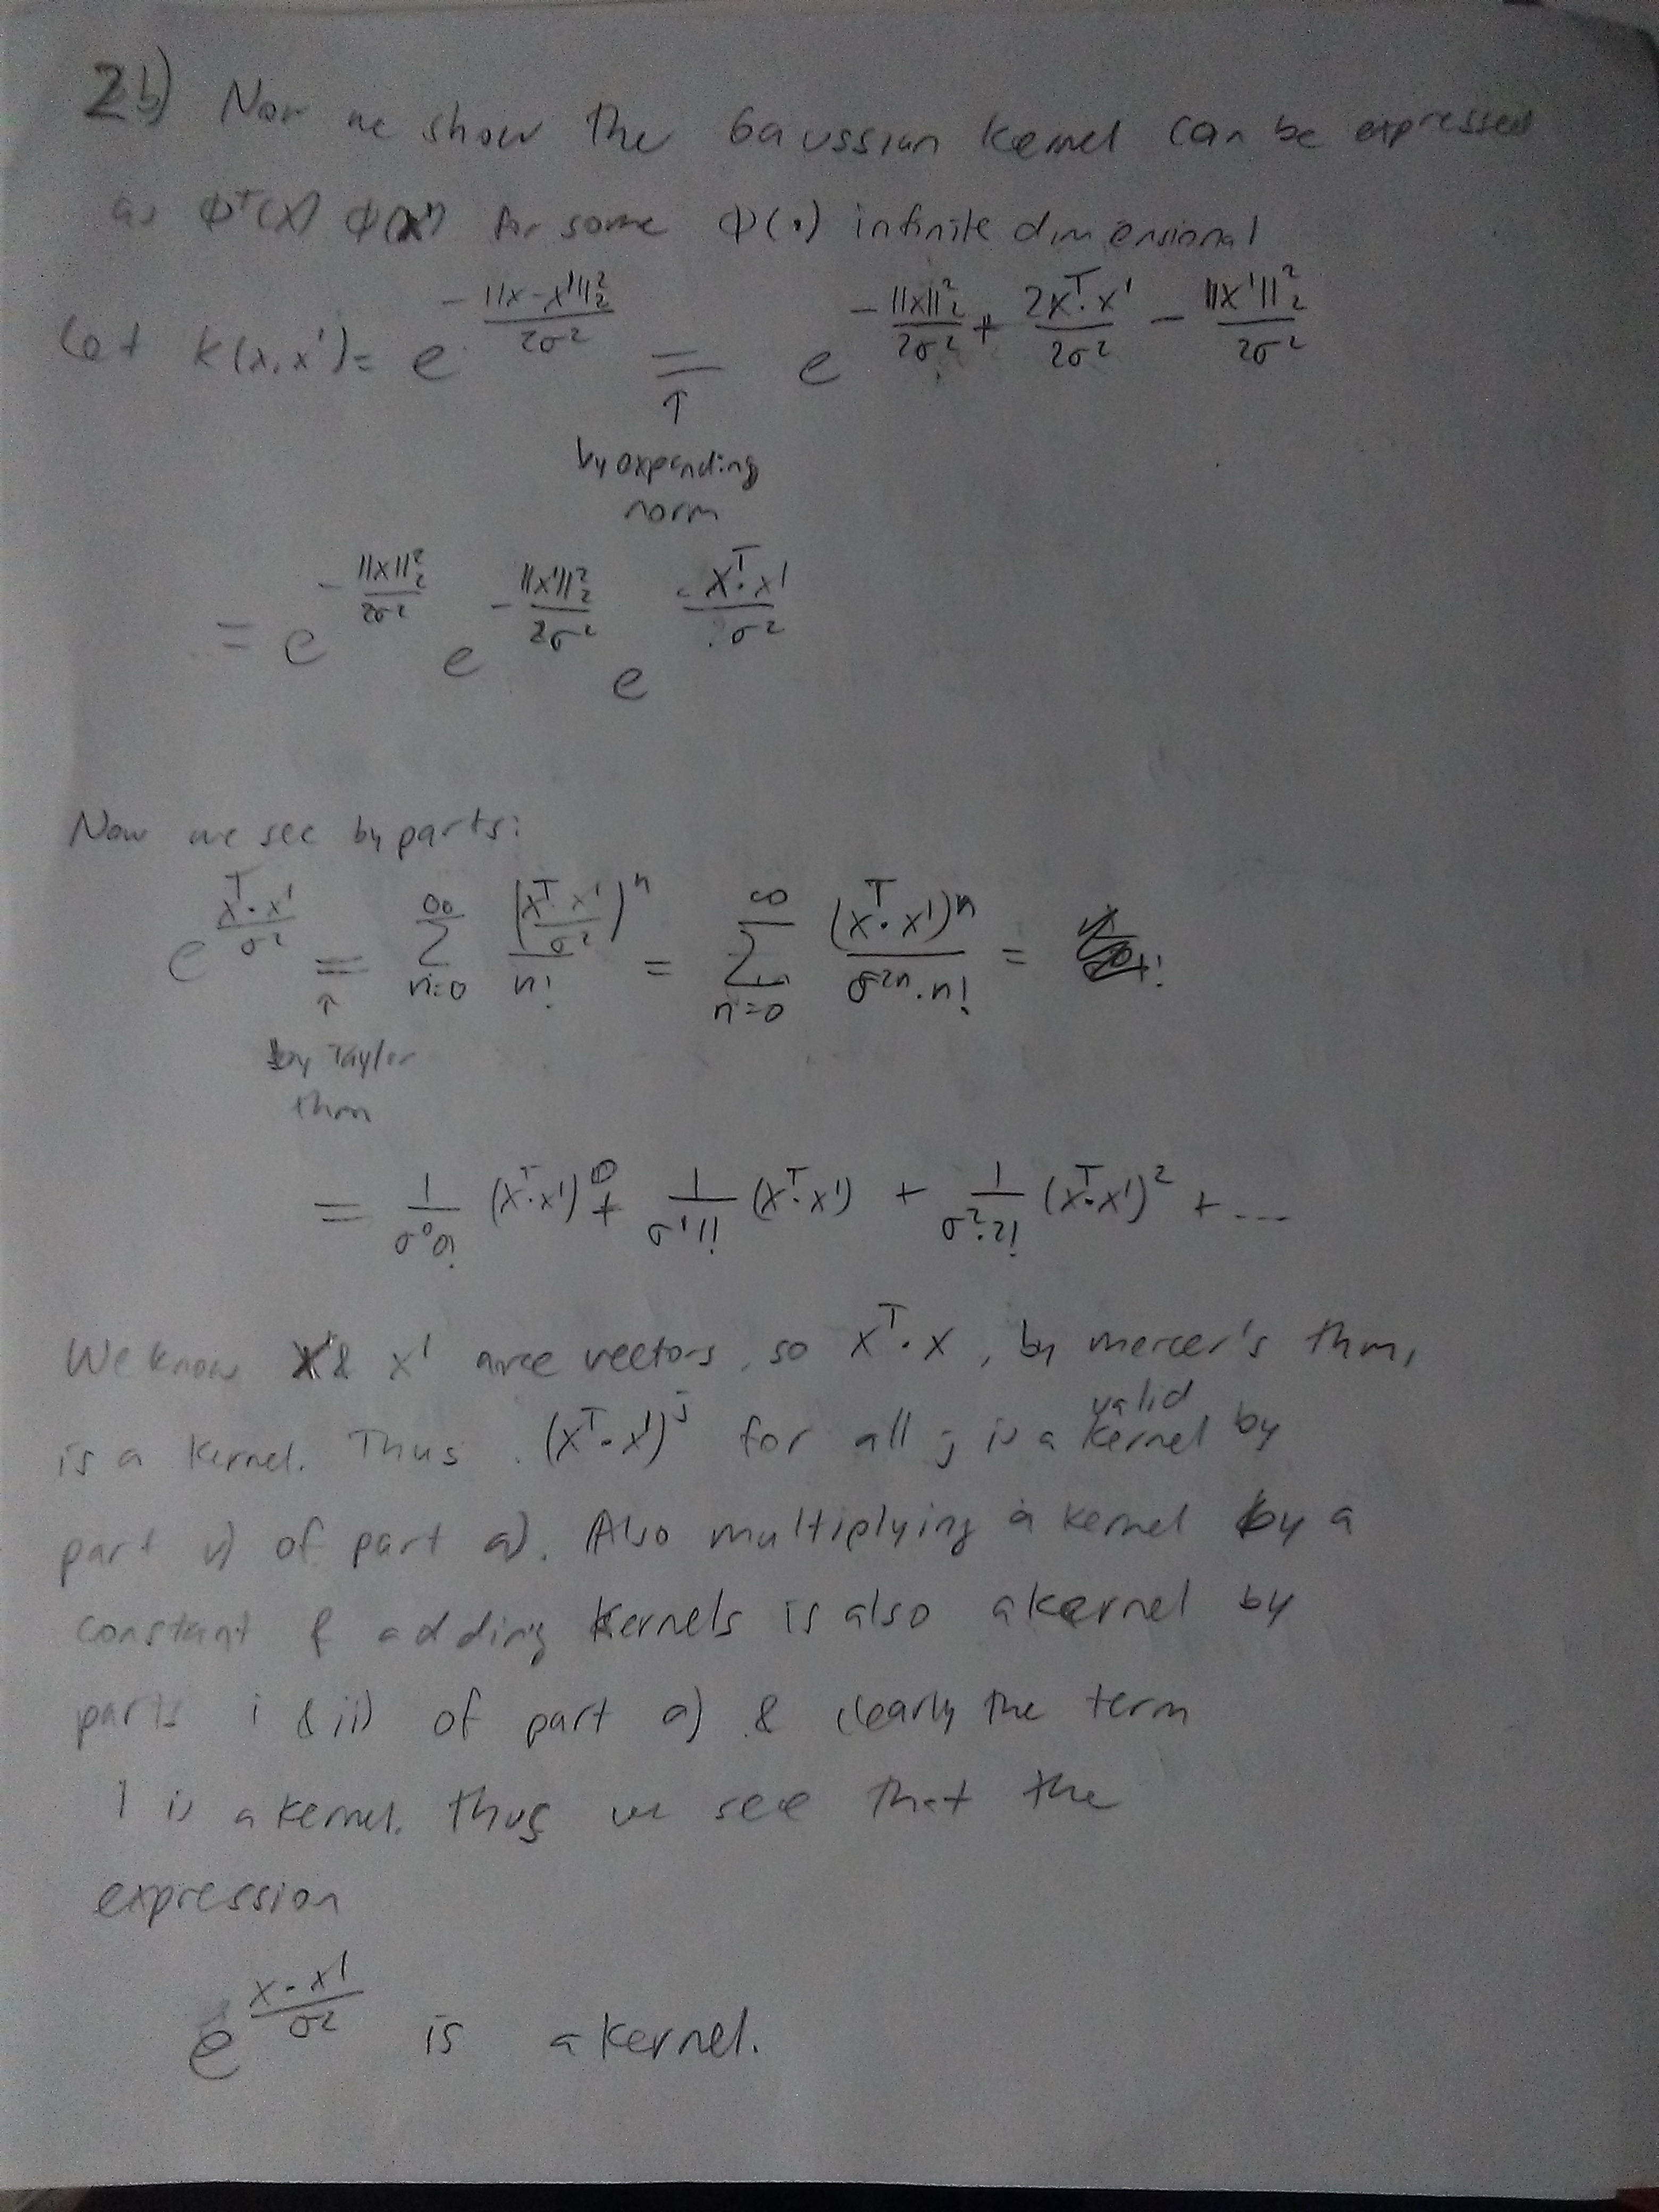
\includegraphics[width=10cm]{hw3_prob2b_1.jpg}
\caption{\textbf{Problem 2b part 1:} Image showing the work for part b of problem 2}
\end{figure}

\begin{figure}[!htbp]
\centering
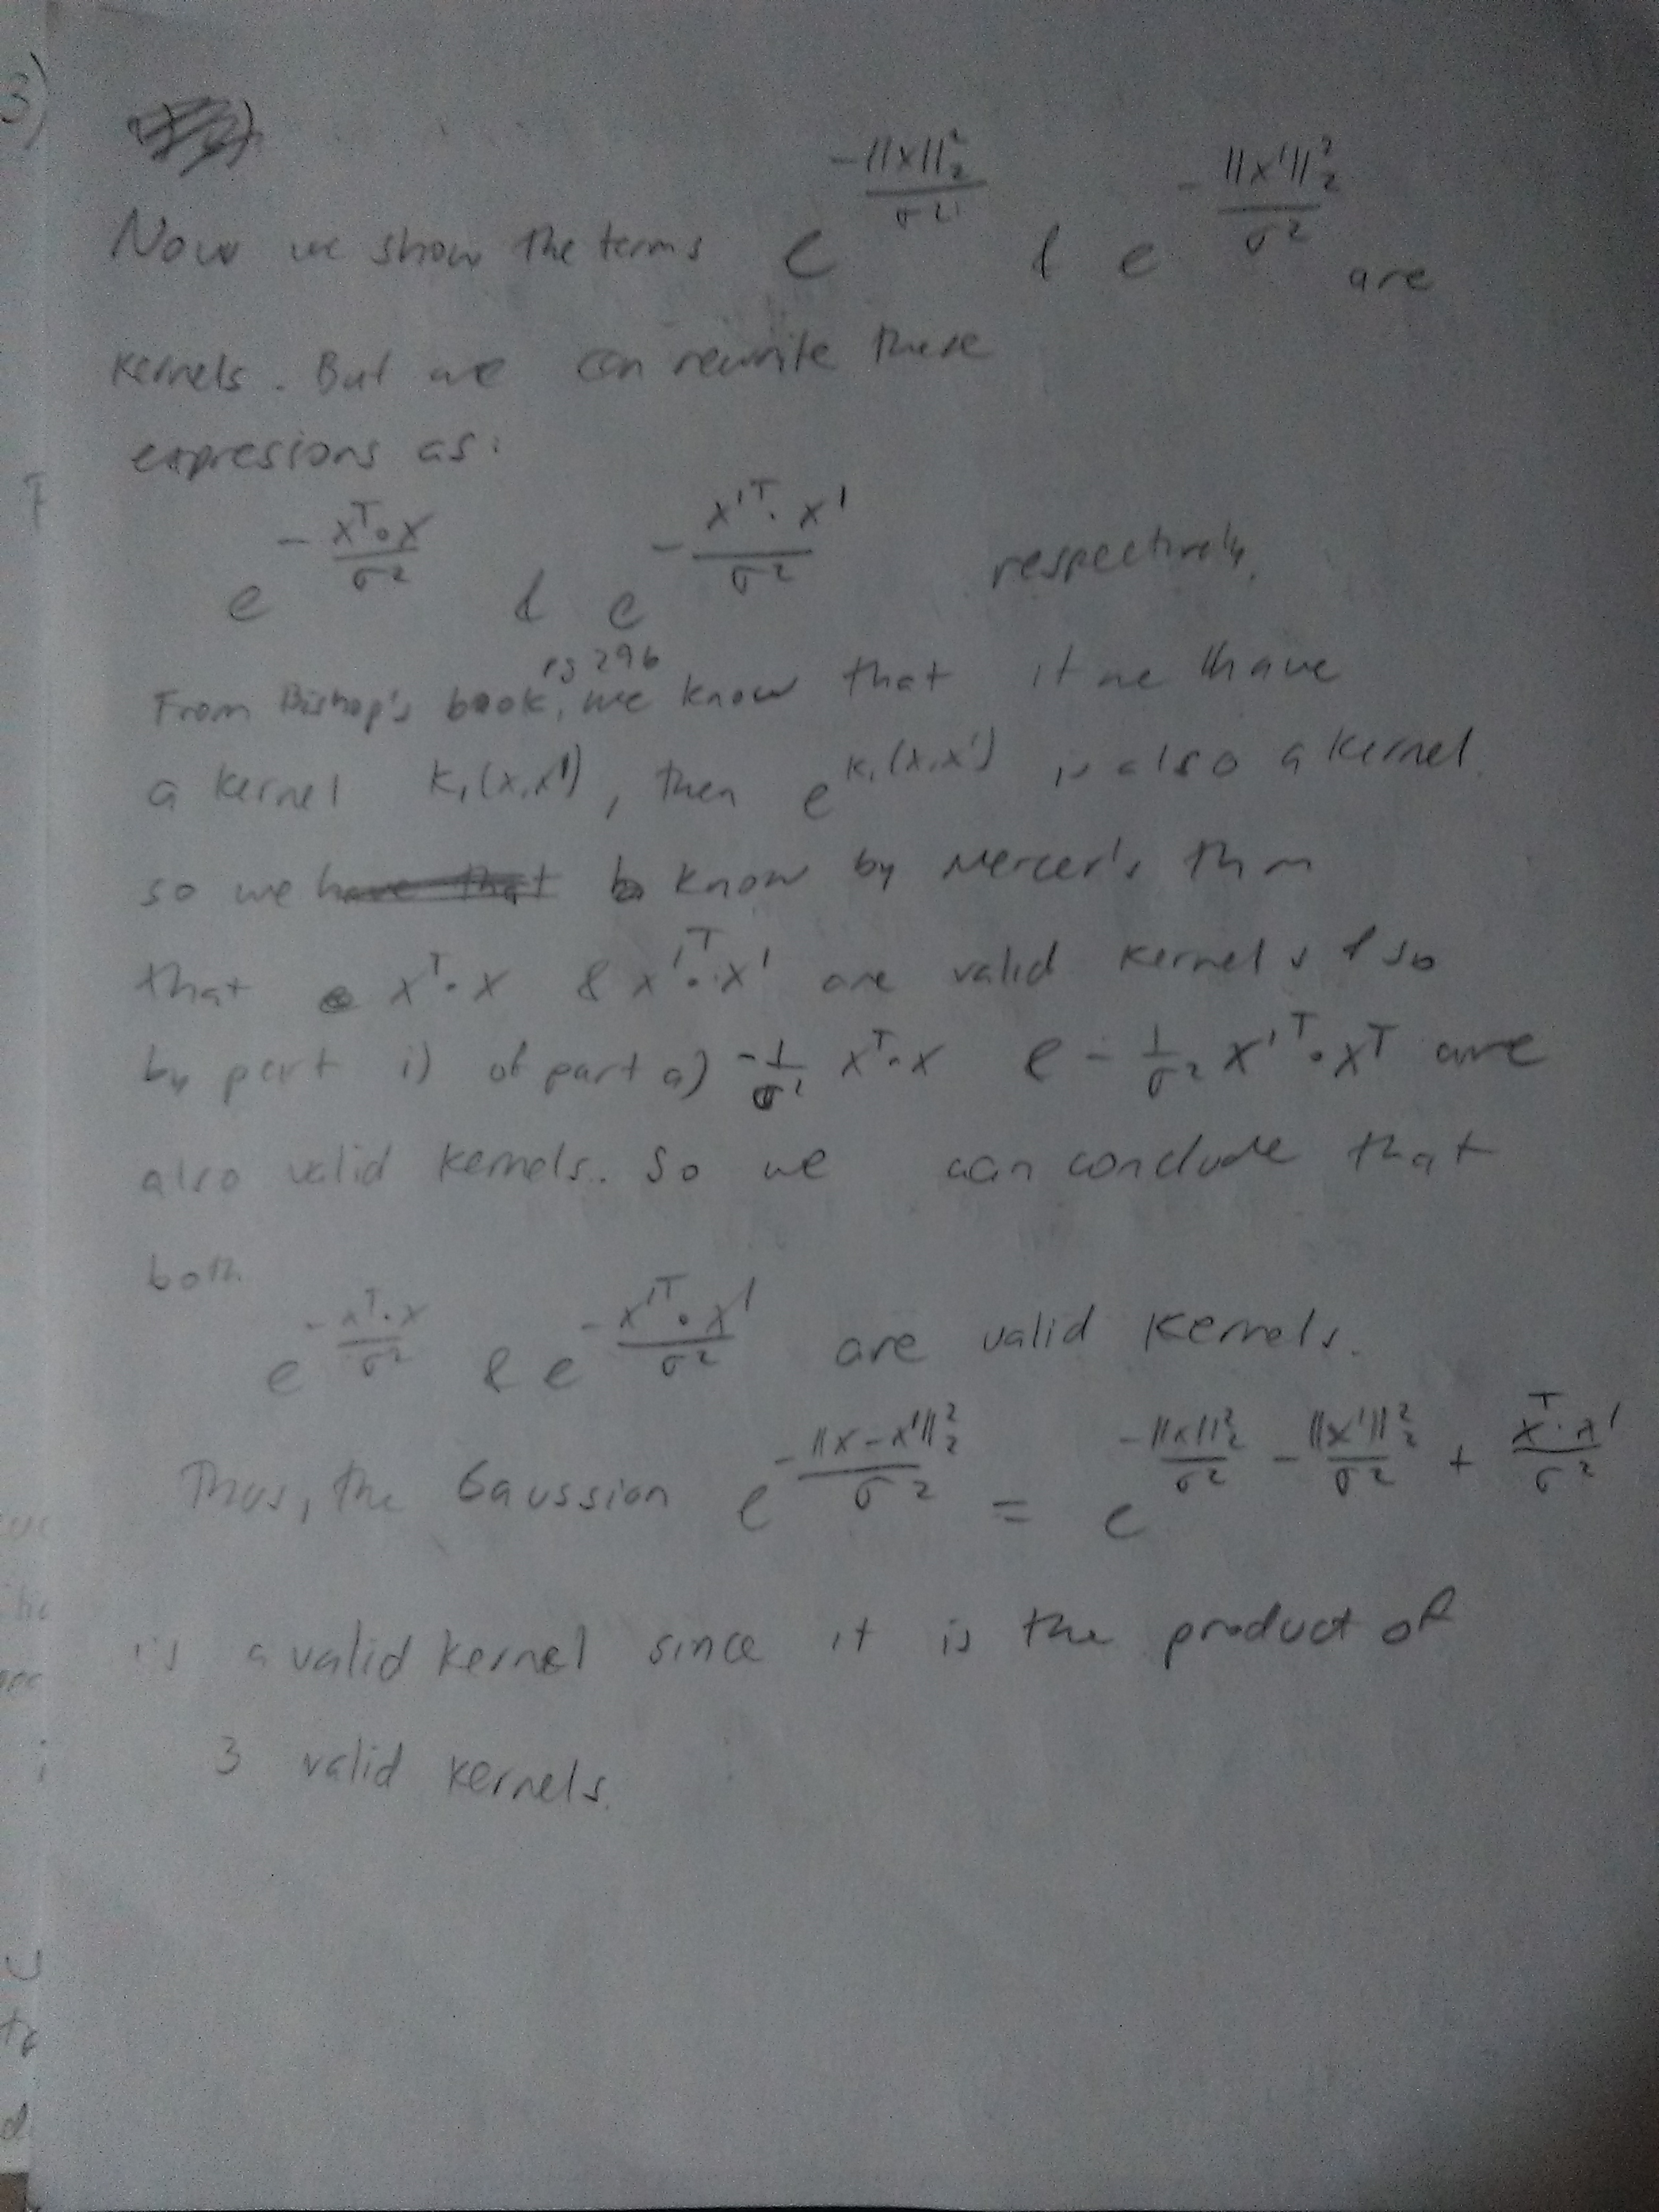
\includegraphics[width=10cm]{hw3_prob2b_2.jpg}
\caption{\textbf{Problem 2b part 2:} Image showing the work for part b of problem 2}
\end{figure}

\end{proof}


\begin{problem}
\normalfont
Problem 3
\end{problem}

\begin{proof}

FOr this problem, first we show our work for \textbf{part a} in the following picture.

\begin{figure}[!htbp]
\centering
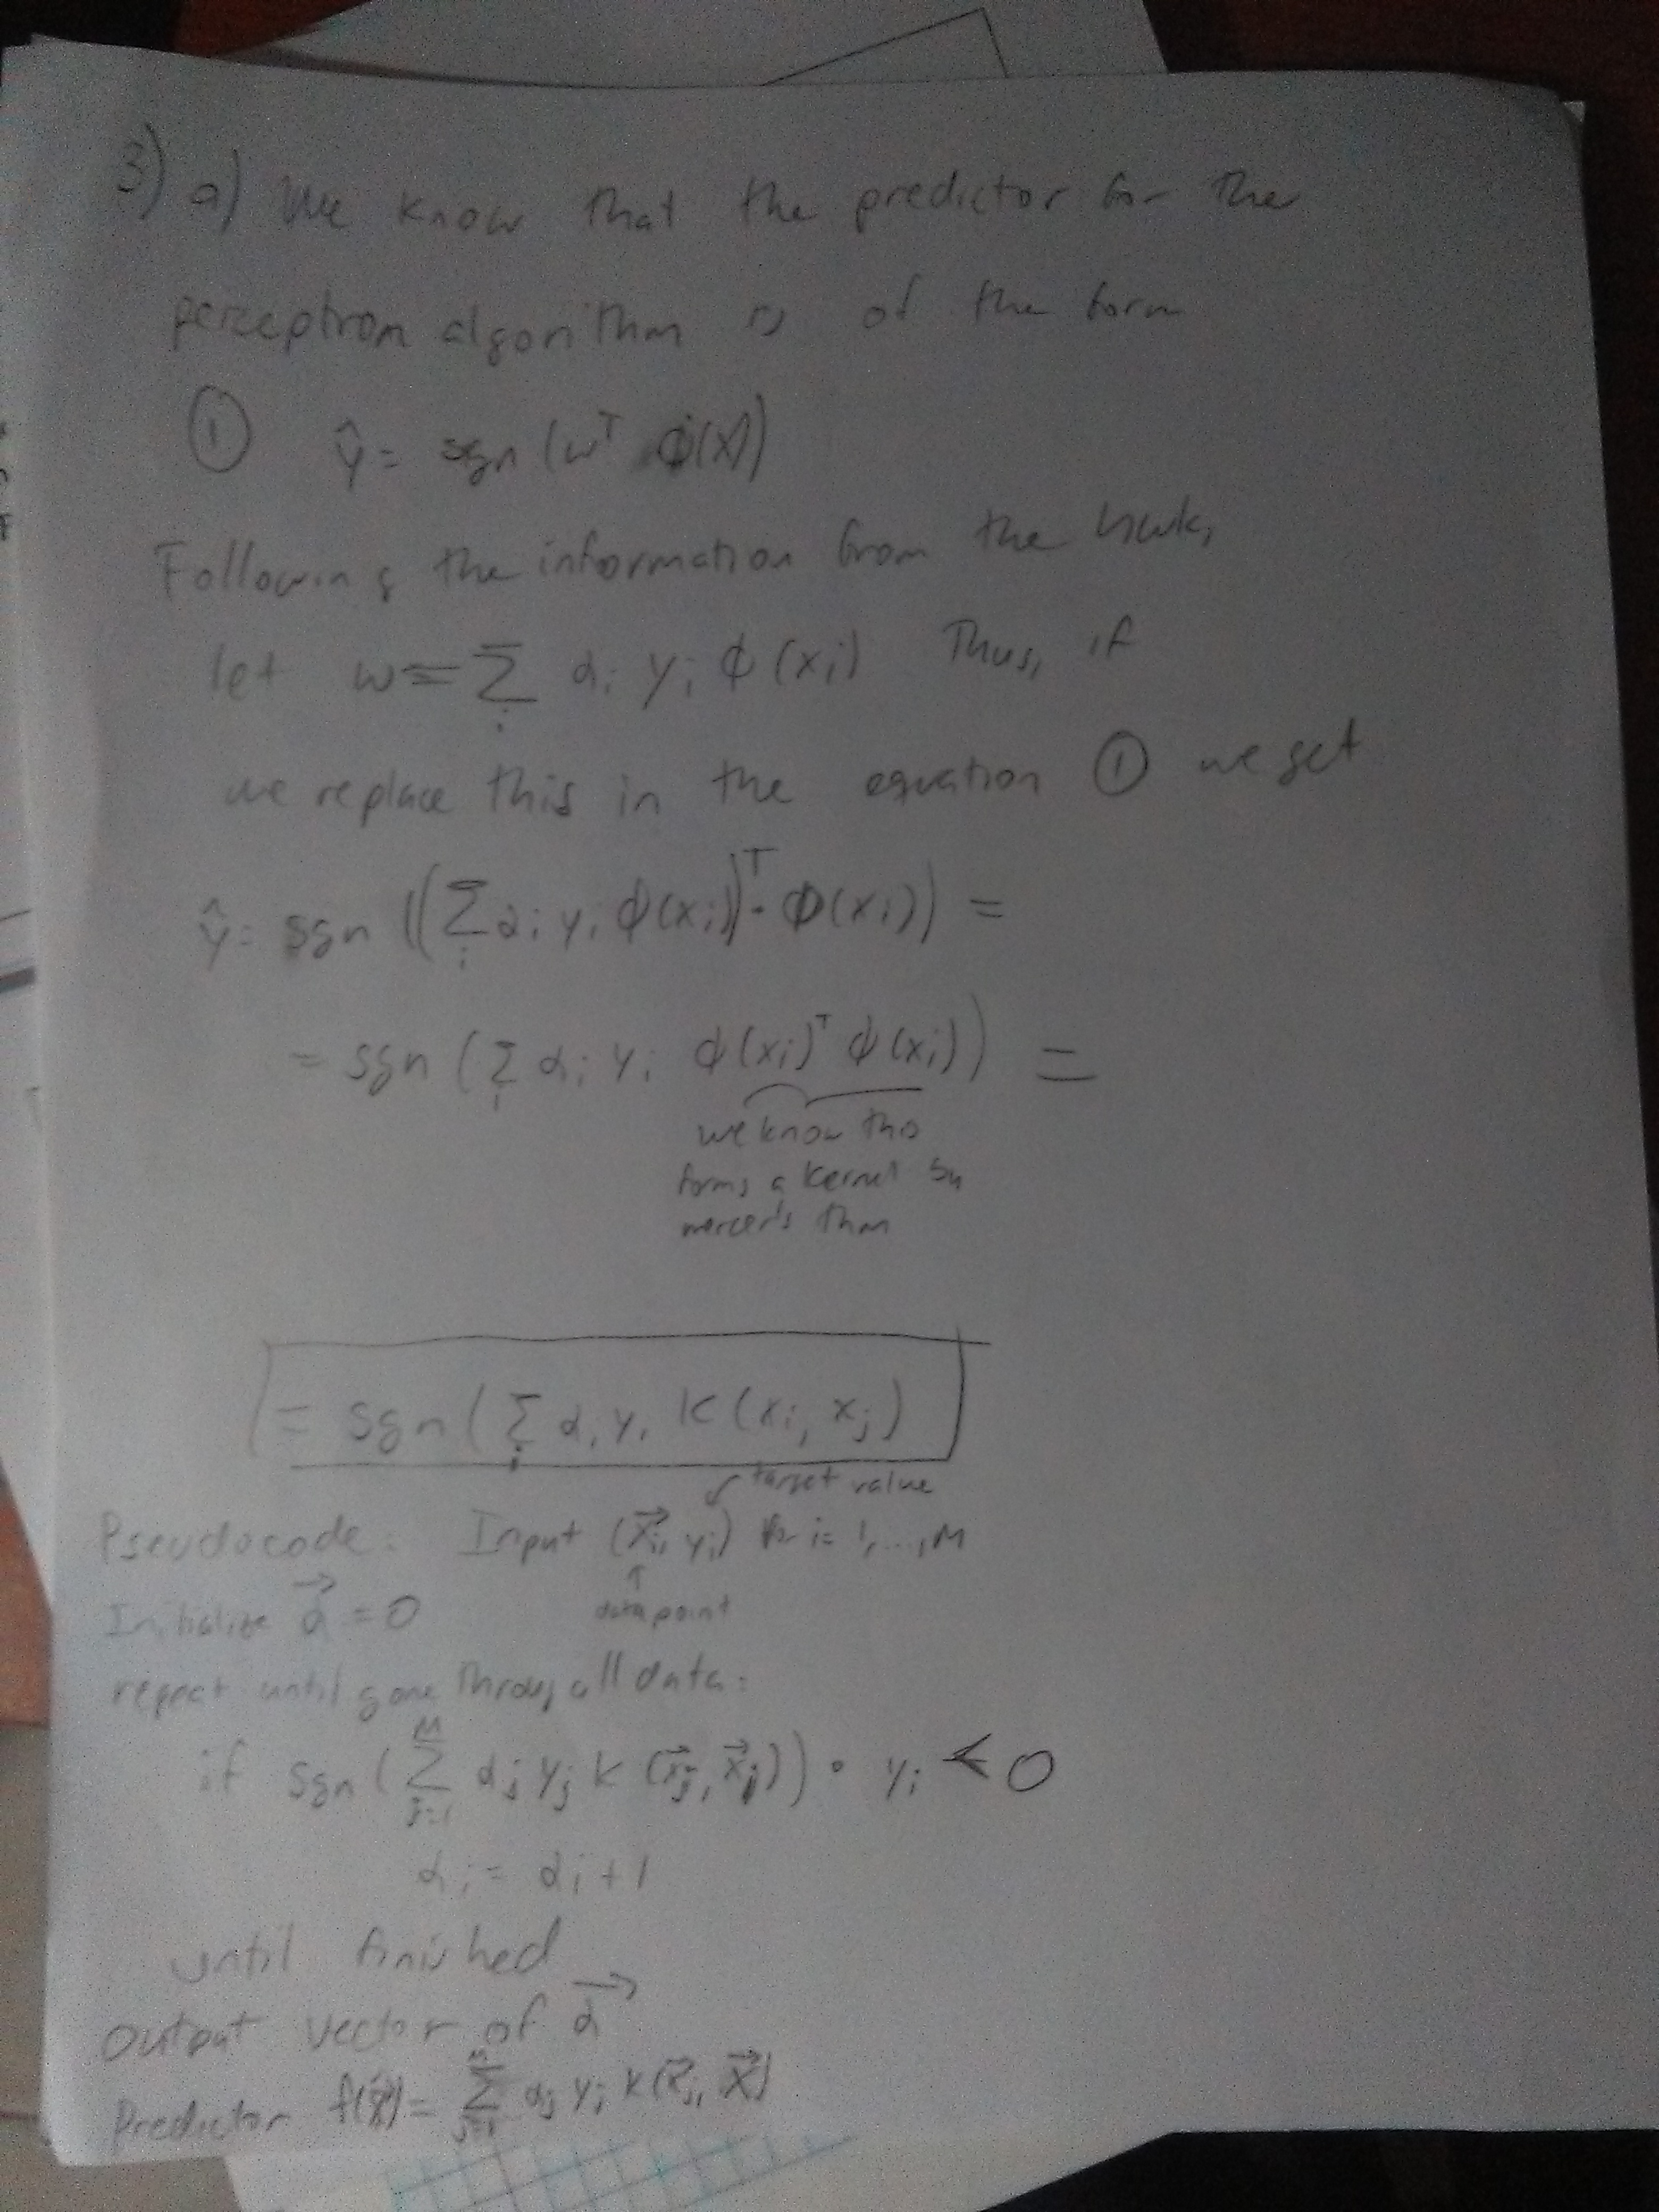
\includegraphics[width=10cm]{hw3_prob3b.jpg}
\caption{\textbf{Problem 3 part a:} Image showing the work for part a of problem 3}
\end{figure}

Now, we show the iamges obtained for part b. The first image shown is just the plot of the data, separated by color. In this plot
blue represents label $-1$ and red represents  label $1$. The next two pictures show a kernel perceptron classifier for when $\sigma = 0.1$ (the second figure below) and $\sigma = 1$ the third figure below. 

\begin{figure}[!htbp]
\centering
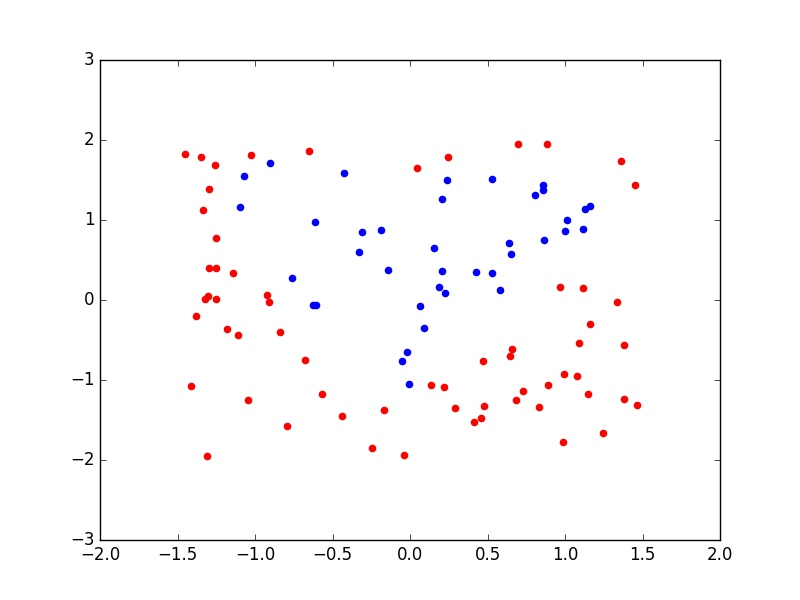
\includegraphics[width=10cm]{hw3_prob3a.jpg}
\caption{\textbf{Problem 3 part b:} Image showing the scatter plot of the data with red color meaning label $1$ and blue color meaning label $-1$}
\end{figure}

\begin{figure}[!htbp]
\centering
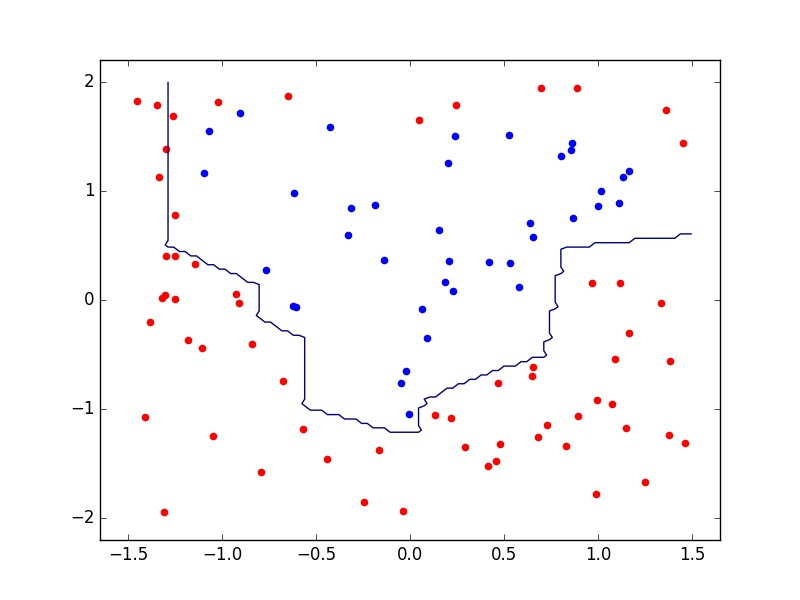
\includegraphics[width=10cm]{hw3_p3_sigma01.jpg}
\caption{\textbf{Problem 3 part b:} Image showing the scatter plot of the data with a kernel perceptron classifier with $\sigma = 0.1$}
\end{figure}




\end{proof}

\begin{problem}
\normalfont
Problem 4
\end{problem}

\begin{proof}

FOr this problem,  we present 2 plots. The \textbf{first plot} we present corresponds to the \textbf{LDA analysis} and the \textbf{second plot} we present corresponds to the\textbf{ QDA analysis.}


\begin{figure}[!htbp]
\centering
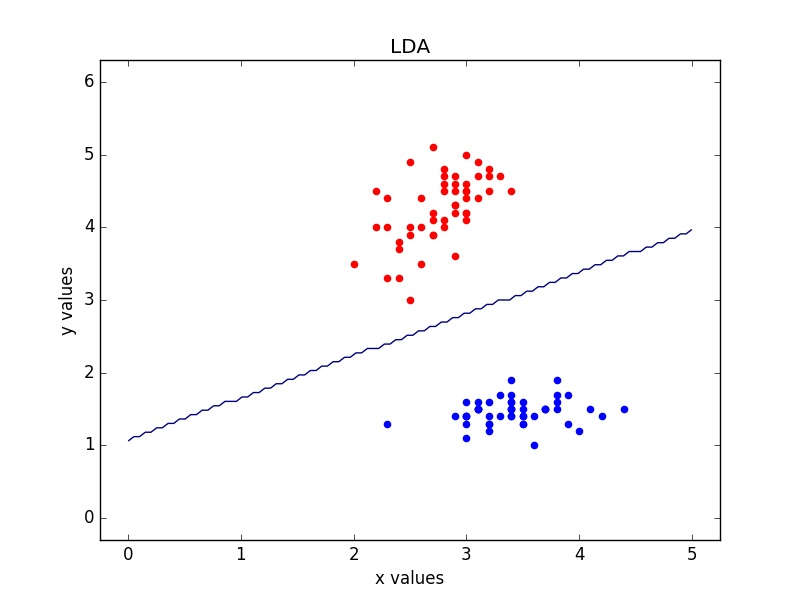
\includegraphics[width=10cm]{hw3_prob4_LDA.jpg}
\caption{\textbf{Problem 4 part LDA:} Image showing the scatter plot of the data with a LDA classifier}
\end{figure}

\begin{figure}[!htbp]
\centering
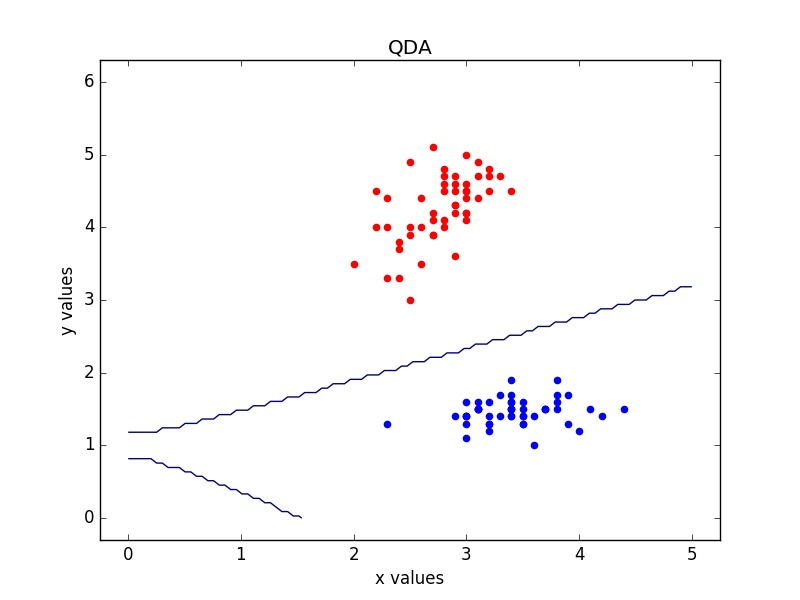
\includegraphics[width=10cm]{hw3_prob4_QDA.jpg}
\caption{\textbf{Problem 4 part QDA:} Image showing the scatter plot of the data with a QDA classifier}
\end{figure}

\end{proof}

\end{document}